\documentclass[]{book}
\usepackage{lmodern}
\usepackage{amssymb,amsmath}
\usepackage{ifxetex,ifluatex}
\usepackage{fixltx2e} % provides \textsubscript
\ifnum 0\ifxetex 1\fi\ifluatex 1\fi=0 % if pdftex
  \usepackage[T1]{fontenc}
  \usepackage[utf8]{inputenc}
\else % if luatex or xelatex
  \ifxetex
    \usepackage{mathspec}
  \else
    \usepackage{fontspec}
  \fi
  \defaultfontfeatures{Ligatures=TeX,Scale=MatchLowercase}
\fi
% use upquote if available, for straight quotes in verbatim environments
\IfFileExists{upquote.sty}{\usepackage{upquote}}{}
% use microtype if available
\IfFileExists{microtype.sty}{%
\usepackage[]{microtype}
\UseMicrotypeSet[protrusion]{basicmath} % disable protrusion for tt fonts
}{}
\PassOptionsToPackage{hyphens}{url} % url is loaded by hyperref
\usepackage[unicode=true]{hyperref}
\hypersetup{
            pdftitle={WorldPop Book of Methods, Vol. I: Gridded Population Estimates},
            pdfauthor={WorldPop, University of Southampton},
            pdfborder={0 0 0},
            breaklinks=true}
\urlstyle{same}  % don't use monospace font for urls
\usepackage{natbib}
\bibliographystyle{plainnat}
\usepackage{color}
\usepackage{fancyvrb}
\newcommand{\VerbBar}{|}
\newcommand{\VERB}{\Verb[commandchars=\\\{\}]}
\DefineVerbatimEnvironment{Highlighting}{Verbatim}{commandchars=\\\{\}}
% Add ',fontsize=\small' for more characters per line
\usepackage{framed}
\definecolor{shadecolor}{RGB}{248,248,248}
\newenvironment{Shaded}{\begin{snugshade}}{\end{snugshade}}
\newcommand{\KeywordTok}[1]{\textcolor[rgb]{0.13,0.29,0.53}{\textbf{#1}}}
\newcommand{\DataTypeTok}[1]{\textcolor[rgb]{0.13,0.29,0.53}{#1}}
\newcommand{\DecValTok}[1]{\textcolor[rgb]{0.00,0.00,0.81}{#1}}
\newcommand{\BaseNTok}[1]{\textcolor[rgb]{0.00,0.00,0.81}{#1}}
\newcommand{\FloatTok}[1]{\textcolor[rgb]{0.00,0.00,0.81}{#1}}
\newcommand{\ConstantTok}[1]{\textcolor[rgb]{0.00,0.00,0.00}{#1}}
\newcommand{\CharTok}[1]{\textcolor[rgb]{0.31,0.60,0.02}{#1}}
\newcommand{\SpecialCharTok}[1]{\textcolor[rgb]{0.00,0.00,0.00}{#1}}
\newcommand{\StringTok}[1]{\textcolor[rgb]{0.31,0.60,0.02}{#1}}
\newcommand{\VerbatimStringTok}[1]{\textcolor[rgb]{0.31,0.60,0.02}{#1}}
\newcommand{\SpecialStringTok}[1]{\textcolor[rgb]{0.31,0.60,0.02}{#1}}
\newcommand{\ImportTok}[1]{#1}
\newcommand{\CommentTok}[1]{\textcolor[rgb]{0.56,0.35,0.01}{\textit{#1}}}
\newcommand{\DocumentationTok}[1]{\textcolor[rgb]{0.56,0.35,0.01}{\textbf{\textit{#1}}}}
\newcommand{\AnnotationTok}[1]{\textcolor[rgb]{0.56,0.35,0.01}{\textbf{\textit{#1}}}}
\newcommand{\CommentVarTok}[1]{\textcolor[rgb]{0.56,0.35,0.01}{\textbf{\textit{#1}}}}
\newcommand{\OtherTok}[1]{\textcolor[rgb]{0.56,0.35,0.01}{#1}}
\newcommand{\FunctionTok}[1]{\textcolor[rgb]{0.00,0.00,0.00}{#1}}
\newcommand{\VariableTok}[1]{\textcolor[rgb]{0.00,0.00,0.00}{#1}}
\newcommand{\ControlFlowTok}[1]{\textcolor[rgb]{0.13,0.29,0.53}{\textbf{#1}}}
\newcommand{\OperatorTok}[1]{\textcolor[rgb]{0.81,0.36,0.00}{\textbf{#1}}}
\newcommand{\BuiltInTok}[1]{#1}
\newcommand{\ExtensionTok}[1]{#1}
\newcommand{\PreprocessorTok}[1]{\textcolor[rgb]{0.56,0.35,0.01}{\textit{#1}}}
\newcommand{\AttributeTok}[1]{\textcolor[rgb]{0.77,0.63,0.00}{#1}}
\newcommand{\RegionMarkerTok}[1]{#1}
\newcommand{\InformationTok}[1]{\textcolor[rgb]{0.56,0.35,0.01}{\textbf{\textit{#1}}}}
\newcommand{\WarningTok}[1]{\textcolor[rgb]{0.56,0.35,0.01}{\textbf{\textit{#1}}}}
\newcommand{\AlertTok}[1]{\textcolor[rgb]{0.94,0.16,0.16}{#1}}
\newcommand{\ErrorTok}[1]{\textcolor[rgb]{0.64,0.00,0.00}{\textbf{#1}}}
\newcommand{\NormalTok}[1]{#1}
\usepackage{longtable,booktabs}
% Fix footnotes in tables (requires footnote package)
\IfFileExists{footnote.sty}{\usepackage{footnote}\makesavenoteenv{long table}}{}
\usepackage{graphicx,grffile}
\makeatletter
\def\maxwidth{\ifdim\Gin@nat@width>\linewidth\linewidth\else\Gin@nat@width\fi}
\def\maxheight{\ifdim\Gin@nat@height>\textheight\textheight\else\Gin@nat@height\fi}
\makeatother
% Scale images if necessary, so that they will not overflow the page
% margins by default, and it is still possible to overwrite the defaults
% using explicit options in \includegraphics[width, height, ...]{}
\setkeys{Gin}{width=\maxwidth,height=\maxheight,keepaspectratio}
\IfFileExists{parskip.sty}{%
\usepackage{parskip}
}{% else
\setlength{\parindent}{0pt}
\setlength{\parskip}{6pt plus 2pt minus 1pt}
}
\setlength{\emergencystretch}{3em}  % prevent overfull lines
\providecommand{\tightlist}{%
  \setlength{\itemsep}{0pt}\setlength{\parskip}{0pt}}
\setcounter{secnumdepth}{5}
% Redefines (sub)paragraphs to behave more like sections
\ifx\paragraph\undefined\else
\let\oldparagraph\paragraph
\renewcommand{\paragraph}[1]{\oldparagraph{#1}\mbox{}}
\fi
\ifx\subparagraph\undefined\else
\let\oldsubparagraph\subparagraph
\renewcommand{\subparagraph}[1]{\oldsubparagraph{#1}\mbox{}}
\fi

% set default figure placement to htbp
\makeatletter
\def\fps@figure{htbp}
\makeatother

\usepackage{booktabs}
\usepackage{amsthm}
\makeatletter
\def\thm@space@setup{%
  \thm@preskip=8pt plus 2pt minus 4pt
  \thm@postskip=\thm@preskip
}
\makeatother

\title{WorldPop Book of Methods, Vol. I: Gridded Population Estimates}
\author{WorldPop, University of Southampton}
\date{2020-11-26}

\begin{document}
\maketitle

{
\setcounter{tocdepth}{1}
\tableofcontents
}
\chapter*{About this book}\label{about-this-book}
\addcontentsline{toc}{chapter}{About this book}

\textbf{Notice: This book is still being drafted! All text is subject to
change. Please do not redistribute it (i.e.~the code, text, images,
tables, etc.) until this notice has been removed.}

This open book provide a guide to WorldPop's gridded population data
sets and the methods used to create them. It was developed by the
WorldPop Research Group within the Department of Geography and
Environmental Science at the University of Southampton. Individual
contributers, collaborators and funders are recognized within each
chapter. Please refer to individual chapters for suggested citations or
cite the whole book as:

\begin{quote}
WorldPop. 2020. \emph{WorldPop Book of Methods, Vol. I: Gridded
Population Estimates}. WorldPop, University of Southampton. 26 November
2020. \url{https://docs.worldpop.org}.
\end{quote}

The source code for the book is available from WorldPop on GitHub:
https://github.com/wpgp/bookworm.

When the notice above is removed, you will be free to copy and
redistribute this book under the CC BY-ND 4.0 license.

\chapter*{Introduction}\label{introduction}
\addcontentsline{toc}{chapter}{Introduction}

This section will introduce you to WorldPop population data sets and
various ways to access them.

\chapter{Gridded Population
Estimates}\label{gridded-population-estimates}

\begin{quote}
\textbf{Note:} This chapter is currently being drafted. To make
suggestions, please raise an
\href{https://github.com/wpgp/bookworm/issues}{issue} in the bookworm
repository. To make direct edits to the source code, please submit a
\href{https://github.com/wpgp/bookworm/pulls}{pull request} to merge
your code with the ``dev'' branch. Include the tag @doug-leasure in your
issues or pull requests to notify Doug.
\end{quote}

WorldPop produces population estimates for every 100 x 100 meter grid
square with national coverage for countries throughout the world.
Gridded data allow end-users to aggregate grid cells to estimate the
total population within any boundaries that meet their needs. It also
provides a consistent grid to facilitate combining data sets like
population, age-sex structure, vaccinations, maternal health, poverty,
etc.

There are three broad categories of methods that WorldPop uses to
produce gridded population estimates:

\begin{enumerate}
\def\labelenumi{\arabic{enumi}.}
\tightlist
\item
  Top-down\\
\item
  Bottom-up\\
\item
  Peanut butter
\end{enumerate}

These approaches require different inputs (i.e.~population data) and the
gridded population estimates that they produce have different
characteristics (Fig. \ref{fig:pop-methods}). Top-down methods require
data from a complete recent census or use other admin totals in each
administrative unit (or other geographic unit). Bottom-up methods
require data from geolocated household surveys that contain a
representative sample of locations across the country. For top-down
approaches, the population totals for adminstrative units are
pre-defined by the input data, whereas in bottom-up approaches, the
population totals are an emergent property that is not pre-defined.

The peanut butter method is different because it relies solely on expert
opinion (rather than hard data) to define the average number of people
per building. The strength of this method lies in the quality of the
high resolution building footprints that are used
\citep{ecopia2020digitize}. This approach may be a good option when
recent and reliable data from a national census and/or household surveys
are not available.

\begin{figure}
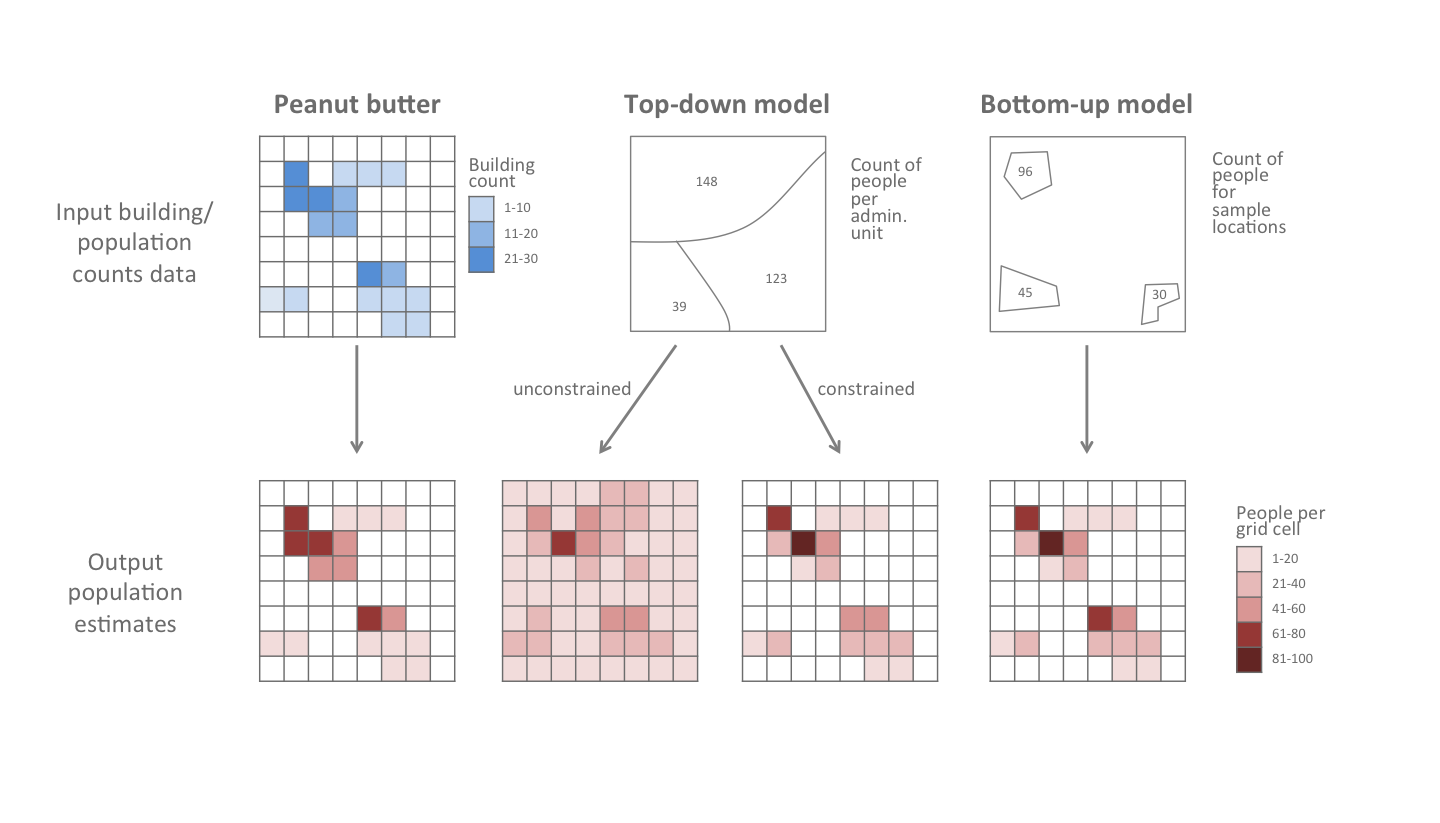
\includegraphics[width=38.28in]{dat/gridded_population_estimates/pop_methods} \caption{Comparison of inputs and outputs for four types of gridded population estimates (from bottom-left to bottom-right): peanut butter, top-down, top-down constrained, and bottom-up.}\label{fig:pop-methods}
\end{figure}

\section{Top-down}\label{top-down}

The top-down method \citep{stevens2015disaggregating} disaggregates
known population totals for each administrative unit (e.g.~states or
local government areas) into 100 m gridded population estimates (Fig.
\ref{fig:pop-methods}). Population totals may be obtained from national
census results projected to the current year (or other years). Gridded
population estimates are created by using machine learning methods
(random forest models) to disaggregate population totals based on
relationships with spatial covariates such as building density, distance
to city center, or intensity of nighttime lights. The disaggregation can
be applied across the entire country or constrained only to areas where
settlements have been mapped.

This is a good approach when recent census totals are available. These
models perform best when accurate census totals are available for the
smallest administrative units. When census results are outdated, this
method relies on projections that can introduce error. Top-down methods
generally do not produce estimates of uncertainty.

See the \protect\hyperlink{top-down-models}{Top-down Models} section for
details.

\section{Bottom-up}\label{bottom-up}

The bottom-up method \citep{wardrop2018spatially, leasure2020national}
uses geolocated household survey data from a sample of locations to fit
statistical models that estimate population sizes for unsampled areas
based on relationships with spatial covariates (Fig.
\ref{fig:pop-methods}). This approach applies customized statistical
models to make the best use of available survey data and to provide
probabilistic estimates of uncertainty.

This is a good approach when recent geolocated household survey data are
available where there has not been a recent or complete national census.
This approach provides robust estimates of uncertainty but requires more
detailed input data and more time to develop the models.

See the \protect\hyperlink{bottom-up-models}{Bottom-up Models} section
for more details.

\section{Peanut Butter}\label{peanut-butter}

The peanut butter method spreads user-provided estimates of people per
building evenly (like peanut butter) among buildings. This is a quick
and simple approach that utilizes high resolution maps of building
footprints, assuming that the same number of people live in each
building across entire regions or settlement types (e.g.~urban and
rural). WorldPop partners with Maxar Technologies, Ecopia.AI, and the
Bill and Melinda Gates Foundation for recent maps of buildings
\citep[\citet{dooley2020gridded}]{ecopia2020digitize}.

This is a good approach when rapid-response population estimates are
needed and no suitable data are available for more data-driven methods.
The peanut butter method ignores spatial variation of people per
building within each region or settlement type and there is often no
objective basis for assessing uncertainty.

The peanut butter method can be applied in aggregation mode or
disaggregation mode:

\begin{itemize}
\item
  \textbf{Aggregation mode} relies on expert opinion to define the
  average number of people per building footprint in each region or
  settlement type.
\item
  \textbf{Disaggregation mode} calculates the average number of people
  per building footprint based on user-provided population totals in
  each region.
\end{itemize}

In both cases, the user-provided estimates of people per building are
mapped to every building footprint. Population totals within each 100 m
grid cell or administrative unit are calculated by summing across all of
the relevant building footprints.

Try the peanut butter method yourself using the peanutButter web
application or the peanutButter R package
\citep{leasure2020peanutButter}.

\section{Comparison of Data}\label{comparison-of-data}

Within these three broad categories, WorldPop develops a variety of
methods for producing gridded population estimates with different
characteristics. Selecting the right population estimation method
depends on project requirements (e.g.~time and resource availability)
and data availability. Table \ref{tab:data-features} provides a
checklist of features for different types of WorldPop gridded population
estimates.

\label{tab:data-features}Comparison of data characteristics for different
types of gridded population estimates. Columns list types of population
estimates and rows provide their characteristics. X marks a feature of a
data set and ? means that a feature is optional. Variations of the
top-down method: 1) Census Projections: basic top-down based on
projected census totals, 2) UN-adjusted: includes a post-hoc adjustment
to match UN population estimates for administrative units, 3)
Constrained: population estimates are constrained to grid cells where
buildings occur (UN-adjustment optional), and 4) Custom: WorldPop
researchers developed a custom top-down model using bespoke data for an
individual country.

Top-down

Peanut Butter

Census Projections

UN-adjusted

Constrained

Custom

Bottom-up Bayesian

Input Population Data

Expert opinion (e.g.~people per building)

X

Population totals for admin units

X

X

X

X

Geolocated household survey data

X

Output Data

Gridded population estimates (\textasciitilde{}100 m)

X

X

X

X

X

X

Sum to match projected census totals

?

X

X

?

Adjusted to match UN admin unit totals

?

X

?

Constrained to buildings

X

X

X

X

Include estimates of uncertainty

X

Access

www.worldpop.org

X

X

X

ftp.worldpop.org

X

X

X

X

X

wopr.worldpop.org

X

X

apps.worldpop.org/woprVision

X

X

apps.worldpop.org/peanutButter

X

 With any of these methods, gridded estimates of total population can be
divided into specific age-sex groups using WorldPop's pre-existing
gridded age-sex proportions. With bottom-up methods, it is also possible
to estimate age-sex proportions directly from household survey data when
it is available. See section \protect\hyperlink{age-sex-mapping}{Age-sex
Mapping} for more information.

\section*{Contributing}\label{contributing}
\addcontentsline{toc}{section}{Contributing}

This chapter was written by Doug Leasure, Claire Dooley,
\emph{{[}contributors, please add your name here{]}}. Funding for the
work described in this chapter was provided by \emph{{[}please add
funders and grant numbers here{]}}.

\section*{Suggested Citation}\label{suggested-citation}
\addcontentsline{toc}{section}{Suggested Citation}

WorldPop. 2020. Introduction: Gridded Population Estimates. In
\emph{WorldPop Book of Methods, Vol. I: Gridded Population Estimates}.
WorldPop, University of Southampton. 26 November 2020,
\url{https://docs.worldpop.org}

\section*{License}\label{license}
\addcontentsline{toc}{section}{License}

This chapter may be redistributed following the terms of a
\href{https://creativecommons.org/licenses/by-nd/4.0/}{Creative Commons
Attribution-NoDerivatives 4.0 International (CC BY-ND 4.0) License}.

\chapter{Data Access}\label{data-access}

\begin{quote}
\textbf{Note:} This chapter is currently being drafted. To make
suggestions, please raise an
\href{https://github.com/wpgp/bookworm/issues}{issue} in the bookworm
repository. To make direct edits to the source code, please submit a
\href{https://github.com/wpgp/bookworm/pulls}{pull request} to merge
your code with the ``dev'' branch. Include the tag @doug-leasure in your
issues or pull requests to notify Doug.
\end{quote}

You can access WorldPop data sets in a variety of ways that could
include downloading individual files from WorldPop.org, downloading in
bulk from the WorldPop FTP server, or creating dynamic links to
population data from your own web server using REST API. The best way to
access population estimates may depend on how you intend to use the data
and the characteristics of the specific data set that you are accessing.

\section{Websites}\label{websites}

WorldPop.org is the central location to access WorldPop data that has
been produced across a range of projects. This includes gridded
population estimates for most countries from the WorldPop Global Project
\citeyearpar[WorldPop et al][]{worldpop2018global} along with gridded
estimates of births, pregnancies, age-sex structure, urban change,
development indicators and other population-related variables.

We are also now developing the WorldPop Open Population Repository to
publish bespoke population data for individual countries, to provide
Bayesian estimates of uncertainty, and to link these data sets to web
applications and other tools.

\section{Web Applications}\label{web-applications}

WorldPop web applications are available from apps.worldpop.org.

These applications allow you to explore population data using
interactive web maps and other tools to maximize the information you get
from population data.

\textbf{Global Demographics Portal}

The WorldPop Demographics app is available at
portal.worldpop.org/demographics. This application allows you to
visualize age-sex proportions estimated for small areas and mapped
across every country.

\textbf{Global Population Data Portal}

The WorldPop Global Data Portal is available from portal.worldpop.org.
This web portal allows you to visualize and download top-down gridded
population estimates for most countries in the world
\citeyearpar[WorldPop et al][]{worldpop2018global}.

\textbf{peanutButter}

The peanutButter application \citep{leasure2020peanutButter} is
available from apps.worldpop.org/peanutButter. This application allows
you to produce gridded population estimates from building footprints
using the peanut butter method. This simple approach requires you to
provide estimates of the average number of people per building in each
settlement type (e.g.~urban and rural). Your estimates are mapped across
buildings using high resolution maps of building footprints
\citep{ecopia2020digitize} that are based on recent satellite imagery.

\textbf{woprVision}

The woprVision application \citep{leasure2020wopr} is available from
apps.worldpop.org/woprVision. This app is an interactive web map that
allows you to query population estimates for specific locations and
demographic groups from the WorldPop Open Population Repository. This
can be used to download population data, query population estimates for
specific locations and demographic groups, and retrieve probabilistic
Bayesian estimates of uncertainty.

\section{FTP Server}\label{ftp-server}

The WorldPop FTP server provides a good resource for downloading files
in bulk. Most data available from the ``DATA'' tab at worldpop.org can
also be downloaded from the ``GIS'' folder on the FTP server.

This includes gridded population estimates produced using the top-down
method for most countries in the world as well as the gridded spatial
covariates used for modelling \citeyearpar[WorldPop et
al.][]{worldpop2018global}.

The ``repo'' folder on the FTP server contains permanent archives of
data sets and code from worldpop.org sub-domains including ``wopr'',
``apps'', and ``docs''. For example, the ``wopr'' sub-directory contains
archived data from wopr.worldpop.org.

\section{GIS Plugins}\label{gis-plugins}

\textbf{wpgpDataAPD}\\
This Esri plugin / ArcPy Python toolbox allows you to download WorldPop
gridded population estimates produced using the top-down method for most
countries globally \citeyearpar[WorldPop et al][]{worldpop2018global}
directly from Esri ArcGIS software. See wpgpDataAPD on GitHub.

\textbf{wpgpDataQPD}\\
This QGIS plugin allows you to download WorldPop gridded population
estimates produced using the top-down method for most countries globally
\citeyearpar[WorldPop et al][]{worldpop2018global} directly from QGIS
software. See wpgpDataQPD on GitHub.

\section{R Packages}\label{r-packages}

\textbf{peanutButter}\\
This package allows you to create your own gridded population estimates
using the peanut butter method and high resolution building footprints
\citep{ecopia2020digitize}. See peanutButter on GitHub.

\textbf{wopr}\\
The wopr package \citep{leasure2020wopr} allows you to download
bottom-up gridded population estimates from the WorldPop Open Population
Repository from your R console and submit spatial queries (i.e.~points
or polygons) to retrieve population estimates for specific locations and
demographic groups with statistical estimates of uncertainty. It also
allows you to run the woprVision web application from your R console.
See wopr on GitHub.

\textbf{wpgpCovariates}\\
This package provides access to gridded spatial covariates
\citeyearpar[WorldPop et al.][]{worldpop2018global} for most countries.
See wpgpCovariates on GitHub.

\textbf{wpgpDownloadR}\\
This package provides access to top-down gridded population estimates
\citeyearpar[WorldPop et al.][]{worldpop2018global} for most countries
from your R console. See wpgpDownloadR on GitHub.

\section{Python Packages}\label{python-packages}

\textbf{wpgpDownloadPy}\\
This Python package provides access to top-down gridded population
estimates \citeyearpar[WorldPop et al.][]{worldpop2018global} from the
Python console. See wpgpDownloadPy on GitHub.

\section{REST API}\label{rest-api}

REST API is a way for computers to communicate with one another to
request data downloads or query databases. Many WorldPop datasets can be
accessed using REST API requests. This makes it possible to
automatically sync remote servers with WorldPop population data and to
develop web applications that use API to query WorldPop servers.

\textbf{WOPR API}\\
This can be used to query bottom-up population estimates from the
WorldPop Open Population Repository. These API endpoints can be used to
download entire data sets for each country or to submit spatial queries
to the WorldPop server to request population estimates for specific
locations and demographic groups. The WOPR API endpoints return Bayesian
estimates of uncertainty for all population estimates. See the chapter
\protect\hyperlink{wopr-api}{WOPR API} for more information.

\textbf{WorldPop API}\\
This can be used to download top-down gridded population estimates from
the WorldPop Global Project \citeyearpar[WorldPop et
al][]{worldpop2018global}. See WorldPop API documentation for more
information.

Contributing

This chapter was written by Doug Leasure, \emph{{[}contributors, please
add your name here{]}}. Funding for the work described in this chapter
was provided by \emph{{[}please add funders and grant numbers here{]}}.

Suggested Citation

WorldPop. 2020. Introduction: Data Access. In \emph{WorldPop Book of
Methods, Vol. I: Gridded Population Estimates}. WorldPop, University of
Southampton. 26 November 2020, \url{https://docs.worldpop.org/bookworm}

\chapter*{Population Mapping Methods}\label{population-mapping-methods}
\addcontentsline{toc}{chapter}{Population Mapping Methods}

This section provides methodological details for the various approaches
that WorldPop has developed for producing gridded population estimates.

\hypertarget{top-down-models}{\chapter{Top-down
Models}\label{top-down-models}}

\begin{quote}
\textbf{Note:} This chapter is currently being drafted. To make
suggestions, please raise an
\href{https://github.com/wpgp/bookworm/issues}{issue} in the bookworm
repository. To make direct edits to the source code, please submit a
\href{https://github.com/wpgp/bookworm/pulls}{pull request} to merge
your code with the ``dev'' branch. Include the tag @bondarenkom in your
issues or pull requests to notify Max and/or @asoriche to notify Ale.
\end{quote}

\section{CIESIN projections}\label{ciesin-projections}

\subsection{Global}\label{global}

\subsection{Individual countries}\label{individual-countries}

\section{UN-adjusted}\label{un-adjusted}

\section{Constrained to building
footprints}\label{constrained-to-building-footprints}

\section{Conclusion}\label{conclusion}

\section*{Contributing}\label{contributing-1}
\addcontentsline{toc}{section}{Contributing}

This chapter was written by \emph{{[}contributors, please add your name
here{]}}. Funding for the work described in this chapter was provided by
\emph{{[}please add funders and grant numbers here{]}}.

\section*{Suggested Citation}\label{suggested-citation-1}
\addcontentsline{toc}{section}{Suggested Citation}

Doe J, \ldots{} . 2020. Population Mapping Methods: Top-down Models. In
\emph{WorldPop Book of Methods, Vol. I: Gridded Population Estimates}.
WorldPop, University of Southampton. 26 November 2020.
\url{https://docs.worldpop.org}

\hypertarget{bottom-up-models}{\chapter{Bottom-up
Models}\label{bottom-up-models}}

\begin{quote}
\textbf{Note:} This chapter is currently being drafted. To make
suggestions, please raise an
\href{https://github.com/wpgp/bookworm/issues}{issue} in the bookworm
repository. To make direct edits to the source code, please submit a
\href{https://github.com/wpgp/bookworm/pulls}{pull request} to merge
your code with the ``dev'' branch. Include the tag @doug-leasure in your
issues or pull requests to notify Doug.
\end{quote}

Bottom-up population modelling methods
\citep{wardrop2018spatially, leasure2020national} use geolocated
household survey data from a sample of locations to fit statistical
models that estimate population sizes for unsampled areas based on
relationships with spatial covariates. WorldPop develops customized
statistical models for individual countries to make the best use of
available survey data and to provide robust estimates of uncertainty.

This is a good approach when there has not been a recent or complete
national census but there are recent geolocated household survey data
available. This approach provides Bayesian estimates of uncertainty but
requires more detailed input data and more time to develop the models.

\section{Input Data}\label{input-data}

Bottom-up methods require a few key types of input data:

\begin{enumerate}
\def\labelenumi{\arabic{enumi}.}
\tightlist
\item
  Population data\\
\item
  Settlement map\\
\item
  Geospatial covariates\\
\item
  Administrative boundaries
\end{enumerate}

\subsection{Population Data}\label{population-data}

Population data for bottom-up methods generally must include counts of
people in clearly defined georeferenced areas. A polygon shapefile with
the boundary of each enumeration area and the total population within
each area is ideal. There are a few potential sources for these data:

\begin{itemize}
\tightlist
\item
  Partial census results\\
\item
  Microcensus surveys designed for population modelling (a random sample
  of locations where enumeration is carried out)\\
\item
  Pre-survey listing data from routine household surveys (e.g.~DHS,
  LSMS, MICS)
\end{itemize}

Point locations of buildings and/or households within enumeration areas
are sometimes collected during census and survey field work. These data
can be very useful because they provide higher resolution information
about population patterns, but they are not required. Pre-survey listing
data can be very useful, especially if surveys were recently conducted
in areas that were inaccessible to census enumerators. If pre-survey
listing data from household surveys are used, additional information
about the site selection will also be required. If the household survey
used a sampling design in which survey locations were selected with
probabilities proportional to population size (PPS), then it will be
necessary to obtain the weights used for PPS sample design.

\subsection{Settlement Map}\label{settlement-map}

A settlement map identifies areas where residential structures occur. It
may also classify areas into settlement types such as urban, peri-urban,
rural, slums, commercial, industrial, etc (see
\protect\hyperlink{settlement-classification}{Settlement
Classification}). This information may be in the form of:

\begin{itemize}
\tightlist
\item
  Building locations (points)\\
\item
  Building footprints (polygons)\\
\item
  Gridded map identifying pixels that contain buildings (raster)
\end{itemize}

These data could be derived from several sources:

\begin{itemize}
\tightlist
\item
  Satellite imagery\\
\item
  Pre-census cartography\\
\item
  Building points and footprints can be purchased commercially
\item
  Gridded derivatives of building footprints are freely available for
  some countries \citep{dooley2020gridded}
\end{itemize}

If there is no classification of settlement types available, building
points or building footprints could be directly used to identify
different settlement types based on the patterns of building locations
\citep{jochem2020classifying, jochem2018identifying}. There are also
freely available global settlement maps, but quality from global data
sets varies strongly among countries, with the smallest settlements
often missing, so this would need to be considered before committing to
any publicly available global settlement map.

Additional data about each building can be very beneficial for
population modelling such as building area, height, or use
(i.e.~residential, commercial, mixed). Classifying individual buildings
as residential or non-residential
\citep{sturrock2018predicting, lloyd2020classifying} can sometimes be
accomplished with existing public data from Open Street Maps and other
sources. While these additional data would improve population estimates,
they are not required.

\subsection{Geospatial Covariates}\label{geospatial-covariates}

Geospatial covariates are spatial data (e.g.~GIS data) with national
coverage that describe any variable that may be correlated with
population densities. There are many suitable datasets that are publicly
available, including some produced by WorldPop for this purpose
\citep{lloyd2019global, dooley2020gridded}.

For example, a digital map of road networks (a line shapefile) could be
used to calculate road densities which may correlate with population
densities. Or, global satellite-derived nighttime lights data sets
(raster files) may correlate with population densities in some areas.
Administrative records could also be useful such as electricity usage
for each administrative unit (polygon shapefile). Locations of public
facilities such as schools (a point shapefile) can also be very
informative. If the number of students attending each school is known,
that would also likely add to the accuracy of population estimates.

There are an almost infinite number of possible geospatial covariates.
Many of them are publicly available, so identifying these data sets is
not necessarily required to initiate population modelling. But,
identifying good quality covariates (i.e.~those that are strongly
correlated to population density) that are comprehensive with national
coverage can significantly improve the accuracy of population estimates.

\subsection{Administrative Boundaries}\label{administrative-boundaries}

Administrative boundaries could include regions, states (provinces),
and/or local government areas. These administrative units are often
nested within one another. Administrative units can be used by the model
as a covariate to improve estimates of population densities.
Administrative units can also be used to summarize model results,
providing population totals for each administrative unit.

\section{Statistical Models}\label{statistical-models}

WorldPop develops customized Bayesian models to make the best use of
available data for specific countries and to accurately quantify
uncertainty associated with the population estimates.

Bayesian models generate population estimates as probability
distributions known as ``posteriors''. You can see examples of posterior
probability distributions for population estimates in the woprVision web
application. We use the mean value of the posterior probability
distribution as the expected value for the population estimate. Variance
around the mean represents uncertainty in the population estimate.

Uncertainty in population estimates may be caused by several factors.
Sometimes uncertainty results from sampling error associated with small
sample sizes (i.e.~not many household survey clusters in the area).
Uncertainty may also represent true variation in population densities
from neighborhood to neighborhood that simply could not be explained by
the covariates in the model. Uncertainty may also be related to the
structure of the statistical model itself. To reduce uncertainty in a
model, you must weigh the cost-benefits for: A) collecting more
household survey data, B) finding better covariates to predict
population densities, or C) revising the model structure. Revising the
model structure is by-far the easiest and this is one reason why the
flexibility of Bayesian models is so important.

\subsection{Software}\label{software}

A quick note about software before we get into the models themselves.
The R programming language for statistical computing \citep{r2020r} is
ideal for fitting Bayesian models. There are a number of software
packages available, but a few that we regularly use are:

\begin{enumerate}
\def\labelenumi{\arabic{enumi}.}
\tightlist
\item
  STAN software \citep{carpenter2017stan} with the rstan R package
  \citep{stan2020rstan}\\
\item
  JAGS software \citep{plummer2003jags} with the runjags R package
  \citep{denwood2016runjags}\\
\item
  INLA R package \citep{lindgren2015bayesian}
\end{enumerate}

If you are new to Bayesian modelling, we recommend starting with STAN
because it provides full flexibility to customize your models, it has
excellent documentation (mc-stan.org) and it is computationally more
efficient than JAGS. If you are already familiar with the BUGS or JAGS
languages, you can build all of the models described below using either
software. If you want to build geostatistical models (see
\protect\hyperlink{geostatistical-models}{Geostatistical Models}), INLA
(R-INLA.org) is the preferred software because it is more
computationally efficient than JAGS or STAN for estimating
high-dimensional spatial covariance parameters, although it is less
flexible for building customized hierarchical models.

\subsection{Simple Model to Start}\label{simple-model-to-start}

A simple linear regression can be written as:

\[
y_i \sim Normal(\mu_i, \sigma) \\
\mu_i = \alpha + \beta x_i
\]

where \(y_i\) is the value of the response variable at location \(i\)
and \(x_i\) is the predictor variable (a.k.a. covariate). These two
variables represent observed data and all of the other variables
represent model parameters that we will estimate using STAN, JAGS, or
INLA (software described above).

\(\mu_i\) is the expected value of the response variable based on the
covariate value \(x_i\) at a given location. It is the mean of the
normal distribution. Random noise that could result in the observed
value being different than the expected value (i.e.~residual variance,
uncertainty) is represented by \(\sigma\) (i.e.~standard deviation). The
regression coeffecient \(\beta\) (i.e.~regression slope) estimates the
effect of the covariate on the expected value, and \(\alpha\)
(i.e.~regression intercept) is the expected value for the response
variable when the covariate is equal to zero.

The first line of the model is the stochastic model (i.e.~it includes
random noise) and the second line is deterministic (i.e.~it always
generates the same output for a given input). The selection of a normal
distribution (a.k.a. Gaussian) in the stochastic portion of the model
should be based on characteristics of the response variable. A normal
distribution represents continuous numbers that can be negative or
positive.

For population modelling, our response variables are counts of people
\(N_i\) that are always positive integers, so we need to choose a more
appropriate stochastic model. We can modify the Gaussian linear
regression above into a Poisson regression:

\begin{equation}
  N_i \sim Poisson( \mu_i ) \\
  log(\mu_i) = \alpha + \beta x_i
  \label{eq:poisson}
\end{equation}

This is a generalized linear model with a log-link function
\citep{mccullagh1989generalized}. The log-link function ensures that
\(\mu_i\) is always positive, and the Poisson distribution produces
positive integers. Now we have an appropriate deterministic regression
and stochastic model for population counts.

\subsection{Bayesian Priors}\label{bayesian-priors}

To implement this model Eq. \eqref{eq:poisson} in a Bayesian context, we
need to define priors for \(\alpha\) and \(\beta\). Priors are
probability distributions that represent our prior knowledge about the
range of possible values for parameters in the model. Priors must be
specified for any ``root node'' parameters, those that do not show up on
the left side of any probability statements in the model. Probability
distributions used as priors are usually very disperse flat priors so
that they do not influence the posterior parameter estimates. In
general, we try to specify priors that are informative enough to define
a realistic range of possible values for the parameter but vague enough
to allow the observed data to have dominating influence on the parameter
estimates.

For the model in Eq. \eqref{eq:poisson}, we could choose uninformative
flat priors: \[
\alpha \sim Uniform(-10, 10) \\
\beta \sim Uniform(-10, 10) 
\] On the log-scale, this is a range from near zero to over 22,000.

Or, we may prefer more informative priors:

\[
\alpha \sim Normal(0, 5) \\
\beta \sim Normal(0, 1) 
\] The relative influence of priors depends on the scale of the response
variable and the structure of the model. It is good practice to test the
relative influence of various priors on the posterior parameter
estimates before making a decision.

In this chapter, we will assume that you understand Bayesian priors and
we will not explicitly specify the priors in our examples unless the
prior selection is noteworthy.

\subsection{Hierarchical Core Model}\label{hierarchical-core-model}

A hierarchical model is one where the output (left side of equation)
from one stochastic model serves as the input (right side) of another.
Building on the Poisson regression in Eq. \eqref{eq:poisson}, we can make
a hierarchical model that incorporates population density \(D_i\):

\begin{equation}
  N_i \sim Poisson( D_i A_i ) \\
  D_i \sim LogNormal( \bar{D}_i, \sigma) \\
  \bar{D}_i = \alpha + \sum_{k=1}^{K} \beta_k x_{i,k}
  \label{eq:likelihood}
\end{equation}

where \(A_i\) is observed data measuring total settled area within
location \(i\). If area is measured in hectares, then \(D_i\) would be
people per hectare. \(\bar{D}_i\) is the expected population density on
the log scale (i.e.~the mean of the log-normal distribution), and
\(\sigma\) is the residual variance term. \(K\) is the total number of
covariates included in the model.

This hierarchical formulation has several advantages over the simple
Poisson regression from Eq. \eqref{eq:poisson}:

\begin{enumerate}
\def\labelenumi{\arabic{enumi}.}
\tightlist
\item
  It adds a residual variance term \(\sigma\) that allows for
  over-dispersion of the Poisson,\\
\item
  Covariates are now predicting population density rather than counts,
  and\\
\item
  The log-normal replaces the log-link function (acting as a stochastic
  log-link).
\end{enumerate}

Over-dispersion means that the model can now accommodate more residual
variance in population counts than could be modelled with a Poisson
distribution alone (because Poisson doesn't have a variance parameter).
In addition, making the covariates predictors of population density
rather than population counts avoids the confounding effect of area. For
example, two locations with identical covariate values and population
densities could have very different population counts if the total
amount of settled area is different. The hierarchical model explicitly
accounts for this multi-level process.

Eq. \eqref{eq:likelihood} will serve as the core likelihood model for many
of the model customizations described below.

\subsection{Age-sex Structure}\label{age-sex-structure}

We can incorporate an age-structured sub-model if the household survey
data contain counts \(M_{i,g}\) of people in each age-sex group \(g\) at
each location \(i\). These data allow us to estimate a population
pyramid (i.e.~proportions of the population in each age-sex group) and
to produce age-sex-specific population estimates. A multinomial model
can be added to Eq. \eqref{eq:likelihood} to achieve this:

\begin{equation}
  M_{i,g} \sim Multinomial(\theta_{r,g}, N_i) \\
  \theta_{r,g} \sim Dirichlet(rep(1,g))
  \label{eq:agesex}
\end{equation}

where \(N_i\) is the total population at location \(i\) from Eq.
\eqref{eq:likelihood}. The population pyramid \(\theta_{r,g}\) is being
estimated independently for each region \(r\) with a flat Dirichlet
prior. The Dirichlet prior enforces the assumptions that individual
elements of \(\theta_{r,g=1:G}\) are between zero and one and that they
sum to one across all age-sex groups \(g\).

\subsection{Random Intercept}\label{random-intercept}

Random effects are regression coefficients (e.g. \(\alpha\) and
\(\beta\) above) that are dependent on other parameters. All of the
regression coefficients shown above were fixed effects because they were
not dependent on other parameters. Models that contain random effects
are sometimes called mixed effects models because they contain fixed and
random effects. Mixed effects models may have random intercepts, random
slopes, or both.

An example of a random intercept in a population model could be a
regression intercept \(\alpha\) (i.e.~average population density) that
is estimated separately for urban and rural areas in a way that accounts
for the correlation between the two. We can adjust Eq.
\eqref{eq:likelihood} to have this random intercept \(\alpha_t\):

\begin{equation}
  N_i \sim Poisson( D_i A_i ) \\
  D_i \sim LogNormal( \bar{D}_i, \sigma) \\
  \bar{D}_i = \alpha_t + \sum_{k=1}^{K} \beta_k x_{i,k} \\
  \alpha_t \sim Normal(\eta, \theta)
\end{equation}

where \(t\) is the settlement type (i.e.~urban or rural) that location
\(i\) belongs to. \(\eta\) and \(\theta\) are the mean and standard
deviation of \(\alpha\) among settlement types. The correlation between
\(\alpha\) for the two settlement types is explicitly modelled because
they are drawn from the same distribution, but these parameter estimates
will still differ based on their fit to the data from each settlement
type. This is a random intercept by settlement type and it can help to
account stratified sampling that household surveys often use to collect
population data.

We can extend this concept to a random intercept by settlement type
\(t\) and region \(r\) to account for additional spatial correlation
where population densities from the same region are more similar to one
another than population densities from different regions. Regions \(r\)
could be defined as states or local government areas. This two-level
random intercept \(\alpha_{t,r}\) (by settlement type and region) could
be included as:

\begin{equation}
  N_i \sim Poisson( D_i A_i ) \\
  D_i \sim LogNormal( \bar{D}_i, \sigma) \\
  \bar{D}_i = \alpha_{t,r} + \sum_{k=1}^{K} \beta_k x_{i,k} \\ 
  \alpha_{t,r} \sim Normal(\breve{\alpha}_{t}, \theta_{t}) \\
  \breve{\alpha}_{t} \sim Normal(\bar{\alpha}, \eta) 
  \label{eq:intercept}
\end{equation}

where \(\breve{\alpha}_{t}\) and \(\theta_{t}\) are the mean and
standard deviation (for each settlement type) of regression intercepts
\(\alpha_{t,r}\) among regions. At the national level, \(\bar{\alpha}\)
and \(\eta\) are the mean and standard deviation for
\(\breve{\alpha}_{t}\).

This hierarchical random intercept can help to account for:\\
- Sampling that is stratified by settlement type, and - Spatial
autocorrelation within regions.

\subsection{Hierarchical Variance}\label{hierarchical-variance}

Similar to the hierarchical random intercept above, we can also use
hierarchical variance by settlement type and region. This allows us to
map uncertainty to see where residual variance is the greatest and
giving more realistic ranges of uncertainty around population estimates
in different regions and settlement types. We could modify Eq.
\eqref{eq:likelihood} to have hierarchical variance \(\sigma_{t,r}\):

\begin{equation}
  N_i \sim Poisson( D_i A_i ) \\
  D_i \sim LogNormal( \bar{D}_i, \sigma_{t,r}) \\
  \bar{D}_i = \alpha + \sum_{k=1}^{K} \beta_k x_{i,k} \\
  \sigma_{t,r} \sim HalfNormal( \breve{\sigma}_t, \theta_t ) \\
  \breve{\sigma}_t \sim HalfNormal( \bar{\sigma}, \eta )
  \label{eq:variance}
\end{equation}

Half-Cauchy distributions are also often recommended for modelling
hierarchical variances rather than the Half-Normal that we have shown
here \citep{gelman2013bayesian}. Hierarchical variances can lead to
convergence issues and care must be taken to specify priors that result
in good convergence without being too influential on the posterior
parameter estimates. It is often necessary to simplify the variance
structure (e.g.~fewer settlement types, or regions, or dropping one
level entirely), especially if the sample size is low in some regions
and/or settlement types.

\subsection{Weighted-likelihood}\label{weighted-likelihood}

Household surveys often implement a weighted sampling design known as
PPS, or Probability Proportional to Size. This means that the
probability of a location being selected for the survey is not random,
it is dependent on the number of people (or households) in that area.
Household surveys use weighted sampling to achieve a representative
sample of households. If they used spatial random sampling, the results
would be biased towards rural areas because urban areas occupy less
space on the landscape.

To use these data for population modelling, it is necessary to account
for the bias that weighted sampling can introduce to avoid
overestimating average population densities. Suppose sample weights
\(w_i\) were used to collect a weighted sample of locations from a
national sampling frame. We can build a weighted-likelihood model that
incorporates these weights to provide unbiased estimates of population
densities. The first step is to calculate inverse weights and scale them
to sum to one:

\begin{equation}
  m_i = \frac{w_i^{-1}}{\sum_{i=1}^1{w_i^{-1}}}
\end{equation}

The scaled inverse weights \(m_i\) (or ``model weights'') are then used
to weight individual samples in the likelihood by adjusting the variance
term \(\sigma_i\):

\begin{equation}
  N_i \sim Poisson( D_i A_i ) \\
  D_i \sim LogNormal( \bar{D}_i , \sigma_i ) \\
  \sigma_i = \sqrt{ \frac{1}{m_i \theta^{-2}} }
  \label{eq:weighted-likelihood}
\end{equation}

where \(\theta\) is an estimated parameter that is a component part of
the variance, together with the model weights \(m_i\). Notice that the
standard deviation for the log-normal \(\sigma_i\) is now
location-specific. This results in unbiased estimates of the mean and
variance because it gives more weight in the likelihood to locations
that had lower probabilities of being included in the sample (e.g.~for
PPS household survey designs this would be locations with fewer people).
The regression model for \(\bar{D}_i\) is not shown but it could be
setup like Eq. \eqref{eq:likelihood}.

The sample weights \(w_i\) are often not known for unsampled areas where
population predictions are needed. Because of this, we need to derive a
weighted average value for the variance term that is not
location-specific:

\[
\bar{\sigma} = \frac{ \sum_{i=1}^I{ \sigma_i \sqrt{m_i} } } { \sum_{i=1}^I{ \sqrt{m_i} } }
\]

This is a weighted average of \(\sigma_i\) across locations \(i\)
(essentially factoring out the model weights \(m_i\)). Model predictions
of population density \(\hat{D}_i\) in locations where sampling weights
\(w_i\) are unknown would be produced from:

\[
\hat{D}_i \sim LogNormal(\bar{D}_i, \bar{\sigma})
\]

\hypertarget{geostatistical-models}{\subsection{Geostatistical
Models}\label{geostatistical-models}}

Geostatistics is a form of spatial statistics that explicitly model a
continuous spatial phenomenon when observations are accurately
georeferenced at particular sites (such as from a GPS location in a
survey). Geostatistical models can help to estimate the outcome in
unobserved locations, with the expectation that nearby locations are
more similar than distant locations. While geostatistical modelling
includes interpolation or smoothing methods such as Kriging, a
model-based geostatistical approach \citep{diggle2016mbg} makes it
possible to incorporate spatial position into a statistical framework
similar to Eq. \eqref{eq:poisson}. The spatial information from the
observations' locations (in addition to observed covariate data) can
improve the accuracy of population estimates. WorldPop has utilised
geostatistical modelling approaches to produce population estimates for
Afghanistan (CITATION), to map the proportion of the population under 5
years of age \citep{alegana2015u5}, produce high-resolution poverty
estimates \citep{steele2017povertymap}, and to estimate vaccination
coverage \citep{utazi2019mapping}.

The general form of the model-based geostatistics framework is a
mixed-effects regression model. This model includes fixed covariate
effects plus a spatially correlated random effect for modelling spatial
variation, to give

\begin{equation}
  N_i \sim Poisson( \mu_i ) \\
  log(\mu_i) = \alpha + \beta x_i + Z(i)
  \label{eq:mbg}
\end{equation}

where \(i\) again indicate locations of observations, but these
locations are taken as a spatial index within a fixed domain
(\(s \in D \subset \R^2\)). \(Z(\cdot)\) is a spatially-continuous
process that can be modelled as a Gaussian random field. Estimating the
characteristics of a Gaussian random field is an important component of
geostatistics, in particular the covariance (\(\Sigma\)) which describes
how the dependence varies as a function of distance between the
observations

Geostatistical models are often implemented using the INLA approach
\citep{krainski2018advanced, lindgren2015bayesian} because estimation of
spatial covariance is very computationally-intensive for MCMC samplers.
Integrated Nested Laplace Approximation (INLA) is a more efficient
alternative to traditional Bayesian MCMC sampling that can provide rapid
approximations of posterior probability distributions. Krainski et al.
\citeyearpar{krainski2018advanced} provide a good introduction to
fitting Bayesian spatial models.

\section{Conclusion}\label{conclusion-1}

Bayesian statistical models used for bottom-up population estimates are
powerful and versatile. We have shown the core strategies that can be
implemented to build appropriate statistical models for various data
sets and applications. These methods are freely available to be built
upon and customized for new applications.

\section*{Contributing}\label{contributing-2}
\addcontentsline{toc}{section}{Contributing}

This chapter was written by Doug Leasure, Andy Tatem, Chris Jochem,
\emph{{[}contributors, please add your name here{]}}. These methods were
developed primarily with funding from the Bill and Melinda Gates
Foundation and the United Kingdom's Foreign, Commonwealth, and
Development Office (OPP1134076, OPP1182408).

\section*{Suggested Citation}\label{suggested-citation-2}
\addcontentsline{toc}{section}{Suggested Citation}

WorldPop. 2020. Population Mapping Methods: Bottom-up Models. In
\emph{WorldPop Book of Methods, Vol. I: Gridded Population Estimates}.
WorldPop, University of Southampton. 26 November 2020.
\url{https://docs.worldpop.org}

\hypertarget{age-sex-mapping}{\chapter{Age-sex
Mapping}\label{age-sex-mapping}}

\begin{quote}
\textbf{Note:} This chapter is currently being drafted. To make
suggestions, please raise an
\href{https://github.com/wpgp/bookworm/issues}{issue} in the bookworm
repository. To make direct edits to the source code, please submit a
\href{https://github.com/wpgp/bookworm/pulls}{pull request} to merge
your code with the ``dev'' branch. Include the tag @bondarenkom in your
issues or pull requests to notify Max.
\end{quote}

\section*{Contributing}\label{contributing-3}
\addcontentsline{toc}{section}{Contributing}

This chapter was written by \emph{{[}contributors, please add your name
here{]}}. Funding for the work described in this chapter was provided by
\emph{{[}please add funders and grant numbers here{]}}.

\section*{Suggested Citation}\label{suggested-citation-3}
\addcontentsline{toc}{section}{Suggested Citation}

Doe J, \ldots{} . 2020. Population Mapping Methods: Age-sex Mapping. In
\emph{WorldPop Book of Methods, Vol. I: Gridded Population Estimates}.
WorldPop, University of Southampton. 26 November 2020.
\url{https://docs.worldpop.org}

\section*{License}\label{license-1}
\addcontentsline{toc}{section}{License}

This report may be redistributed following the terms of a
\href{https://creativecommons.org/licenses/by-nd/4.0/}{Creative Commons
Attribution-NoDerivatives 4.0 International (CC BY-ND 4.0) License}.

\hypertarget{settlement-classification}{\chapter{Settlement
Classification}\label{settlement-classification}}

\begin{quote}
\textbf{Note:} This chapter is currently being drafted. To make
suggestions, please raise an
\href{https://github.com/wpgp/bookworm/issues}{issue} in the bookworm
repository. To make direct edits to the source code, please submit a
\href{https://github.com/wpgp/bookworm/pulls}{pull request} to merge
your code with the ``dev'' branch. Include the tag @wjochem in your
issues or pull requests to notify Chris J.
\end{quote}

\section{Point-based}\label{point-based}

\section{Polygon-based}\label{polygon-based}

\section{Building-type}\label{building-type}

\section{Conclusion}\label{conclusion-2}

\section*{Contributing}\label{contributing-4}
\addcontentsline{toc}{section}{Contributing}

This chapter was written by \emph{{[}contributors, please add your name
here{]}}. Funding for the work described in this chapter was provided by
the Bill and Melinda Gates Foundation and the United Kingdom Foreign,
Commonwealth \& Development Office as part of the GRID3 project
(OPP1182408, OPP1182425).

\section*{Suggested Citation}\label{suggested-citation-4}
\addcontentsline{toc}{section}{Suggested Citation}

Doe J, \ldots{} . 2020. Population Mapping Methods: Settlement
Classification. In \emph{WorldPop Book of Methods, Vol. I: Gridded
Population Estimates}. WorldPop, University of Southampton.
\url{https://docs.worldpop.org}.

\section*{License}\label{license-2}
\addcontentsline{toc}{section}{License}

This report may be redistributed following the terms of a
\href{https://creativecommons.org/licenses/by-nd/4.0/}{Creative Commons
Attribution-NoDerivatives 4.0 International (CC BY-ND 4.0) License}.

\chapter*{Bespoke Population Models}\label{bespoke-population-models}
\addcontentsline{toc}{chapter}{Bespoke Population Models}

This section describes methods developed for specific country contexts.

\chapter{Nigeria (v1)}\label{nigeria-v1}

\begin{quote}
\textbf{Note:} This chapter is currently being drafted. To make
suggestions, please raise an
\href{https://github.com/wpgp/bookworm/issues}{issue} in the bookworm
repository. To make direct edits to the source code, please submit a
\href{https://github.com/wpgp/bookworm/pulls}{pull request} to merge
your code with the ``dev'' branch. Include the tag @doug-leasure in your
issues or pull requests to notify Doug.
\end{quote}

\textbf{Note:} The gridded population estimates for Nigeria
\citep{worldpop2019bottom-up, worldpop2020bottom-up} are available from
the WorldPop Open Population Repository and they can be explored on a
map using the woprVision web application (select ``NGA v1.2'').

\begin{figure}
\centering
\includegraphics[width=1.00000\textwidth,height=6.25000in]{./dat/NGAv1/NGA_population_v1_x_methods.pdf}
\caption{\href{https://doi.org/10.1073/pnas.1913050117}{Proceedings of
the National Academy of Sciences} \citep{leasure2020national}}
\end{figure}

\section*{Contributing}\label{contributing-5}
\addcontentsline{toc}{section}{Contributing}

Funding for the work described in this chapter was provided by the Bill
and Melinda Gates Foundation and the United Kingdom Foreign,
Commonwealth \& Development Office as part of the GRID3 project
(OPP1182408, OPP1182425).

\chapter{Ghana (v1)}\label{ghana-v1}

A Bayesian approach to produce 100 m gridded population estimates using
census microdata and recent building footprints

WorldPop, University of Southampton

16 November 2020

\begin{quote}
\textbf{Note:} The gridded population estimates for Ghana described in
this chapter are available from the WorldPop Open Population Repository
and they can be explored on a map using the woprVision web application
(select ``GHA v1.0''). This chapter was originally published as a report
with appendices and supplemental data \citep{leasure2020approach}.
\end{quote}

\section{Introduction}\label{introduction-1}

Gridded population estimates can provide an important resource for
planning government services, housing and population censuses, health
and education initiatives, household surveys and other programes in
situations when their are no recent census data available. Gridded
population estimates can be aggregated to estimate total populations for
custom areas suited to individual project goals. WorldPop uses two
general approaches for producing gridded population estimates: bottom-up
and top-down \citep{wardrop2018spatially}.

Top-down methods \citep{stevens2015disaggregating} dissaggregate known
population totals for administrative units into gridded population
estimates at higher spatial resolution (e.g.~100 m). This approach is
best for situations when reliable population totals for administrative
units are available from a recent census or census projections. The
population totals are dissaggregated based on relationships with gridded
geospatial covariates that are mapped consistently across an entire
study area or region of interest such as nighttime lights, impervious
surfaces, and distance to city centers. Top-down approaches are not
reliable when population totals from a recent census are not available
and population projections are not reliable due to population
displacement, time since the last census, or other reasons.

Bottom-up methods \citep{leasure2020national} use population counts from
a sample of locations (e.g.~from household surveys) to produce gridded
population estimates with full national coverage. This approach is best
for situations when population totals from census are not available but
recent household survey data are available with full enumeration of
people in a sample of clearly defined survey locations. Like the
top-down method, populations are estimated based on relationships with
gridded geospatial covariates. Bottom-up methods are often based on
Bayesian statistical models that provide robust estimates of
uncertainty, whereas top-down models based on machine learning models
\citep{stevens2015disaggregating} do not provide any confidence bounds
on population estimates. One challenge with the bottom-up approach is
that it requires geolocated household survey data that can be difficult
to access due to privacy safeguards that must be put in place.

A method is needed that can produce robust gridded population estimates
in situations when recent census data and geolocated household survey
data are both unavailable. There are publicly available anonymized
household survey data without specific location information that could
be used for this purpose (e.g.~IPUMS, DHS). Increasing availability of
building footprints mapped from satellite imagery also provide a
valuable source of information. A statistical method that measures
statistical uncertainty for population estimates would be needed because
the inherent uncertainty in population data that are not geolocated will
likely produce population estimates with wide confidence intervals that
would be important for end users to be aware of.

Our goal here was to develop a new Bayesian statistical model to
estimate the number of households per building and people per household
at sub-national spatial scales. We prioritized the use of publicly
available data so that the method could be replicated across countries
more easily. We demonstrated this new approach with a case study to
produce gridded population estimates for Ghana. Our aim was to produce:

\begin{enumerate}
\def\labelenumi{\arabic{enumi}.}
\tightlist
\item
  100 meter gridded population estimates with national coverage,
\item
  Estimates of age-sex structure by region and settlement type,
\item
  Estimates of people per household by geographic unit and settlement
  type,
\item
  Estimates of households per building by geographic unit and settlement
  type, and
\item
  Robust estimates of uncertainty for population estimates (and other
  parameters) at any spatial scale.
\end{enumerate}

\section{Methods}\label{methods}

The total population for an area can be described as a function of the
number of buildings:

\[
population = buildings \times \frac{households}{building} \times \frac{people}{household}
\] We develop this equation into a hierarchical statistical model below,
but first we will describe the sources of information needed to inform
the parameters on the right side of the equation.

\subsection{Data}\label{data}

\textbf{Building footprints.} We used rasterized counts of buildings
within approximately 100 m grid cells across Ghana
\citep{dooley2020gridded}. These were derived from building footprints
for sub-saharan Africa that were extracted from from recent
high-resolution satellite imagery \citep{ecopia2020digitize} (modal year
= 2018, range = 2009 to 2019).

\textbf{Census microdata.} We used microdata samples from the 2010 Ghana
census that were publicly available from IPUMS International
\citep{mpc2019integrated}. This provides a count of the number of people
from thousands of housing units with representative national coverage.
Each household record is geo-tagged to geographic areas nested within
larger regions. These level 1 and level 2 geographic boundaries (Fig.
\ref{fig:map}) were available for download from IPUMS International
\citep{mpc2019integrated}.

There were no GPS coordinates associated with these household-level
survey data for privacy reasons. The absence of specific location
information is one of the primary challenges to overcome with the
statistical model. Geospatial covariates that are usually fundamental
for bottom-up statistical models
\citep{wardrop2018spatially, leasure2020national} cannot be used here
because we do not know the exact locations of the household surveys.

We used this to estimate the average number of people per household
within sub-national geographic units. We also used these data to
estimate the demographic composition of the populations in these areas
by age and sex. We will assume that these parameters have not changed
since 2010 when the census was conducted.

\textbf{Population totals.} We used population totals for level 3
administrative units that were projected to the year 2018 from the last
census \citep{worldpop2018globala}. We also used the level 3
administrative boundaries used for those projections
\citep{worldpop2018globalb} (Fig. \ref{fig:map}).

We used this to estimate the average number of housing units per
building. We used projections to the year 2018 to match the year of the
building footprints.

\textbf{Settlement type.} We used the urban and rural classifications of
enumeration areas from the 2010 Ghana census \citep{gss2010census}. We
summarized the original three settlement types into urban and rural
classes based on guidance from Ghana Statistical Services. We assumed
that this was the same urban and rural classification reported in the
census microdata from IPUMS International \citep{mpc2019integrated}.

Maps of settlement types, administrative boundaries, and IPUMS
geographic regions (Fig. \ref{fig:map}) were rasterized to a 100 m
mastergrid matching the building footprints rasters
\citep{dooley2020gridded}.

\begin{figure}

{\centering 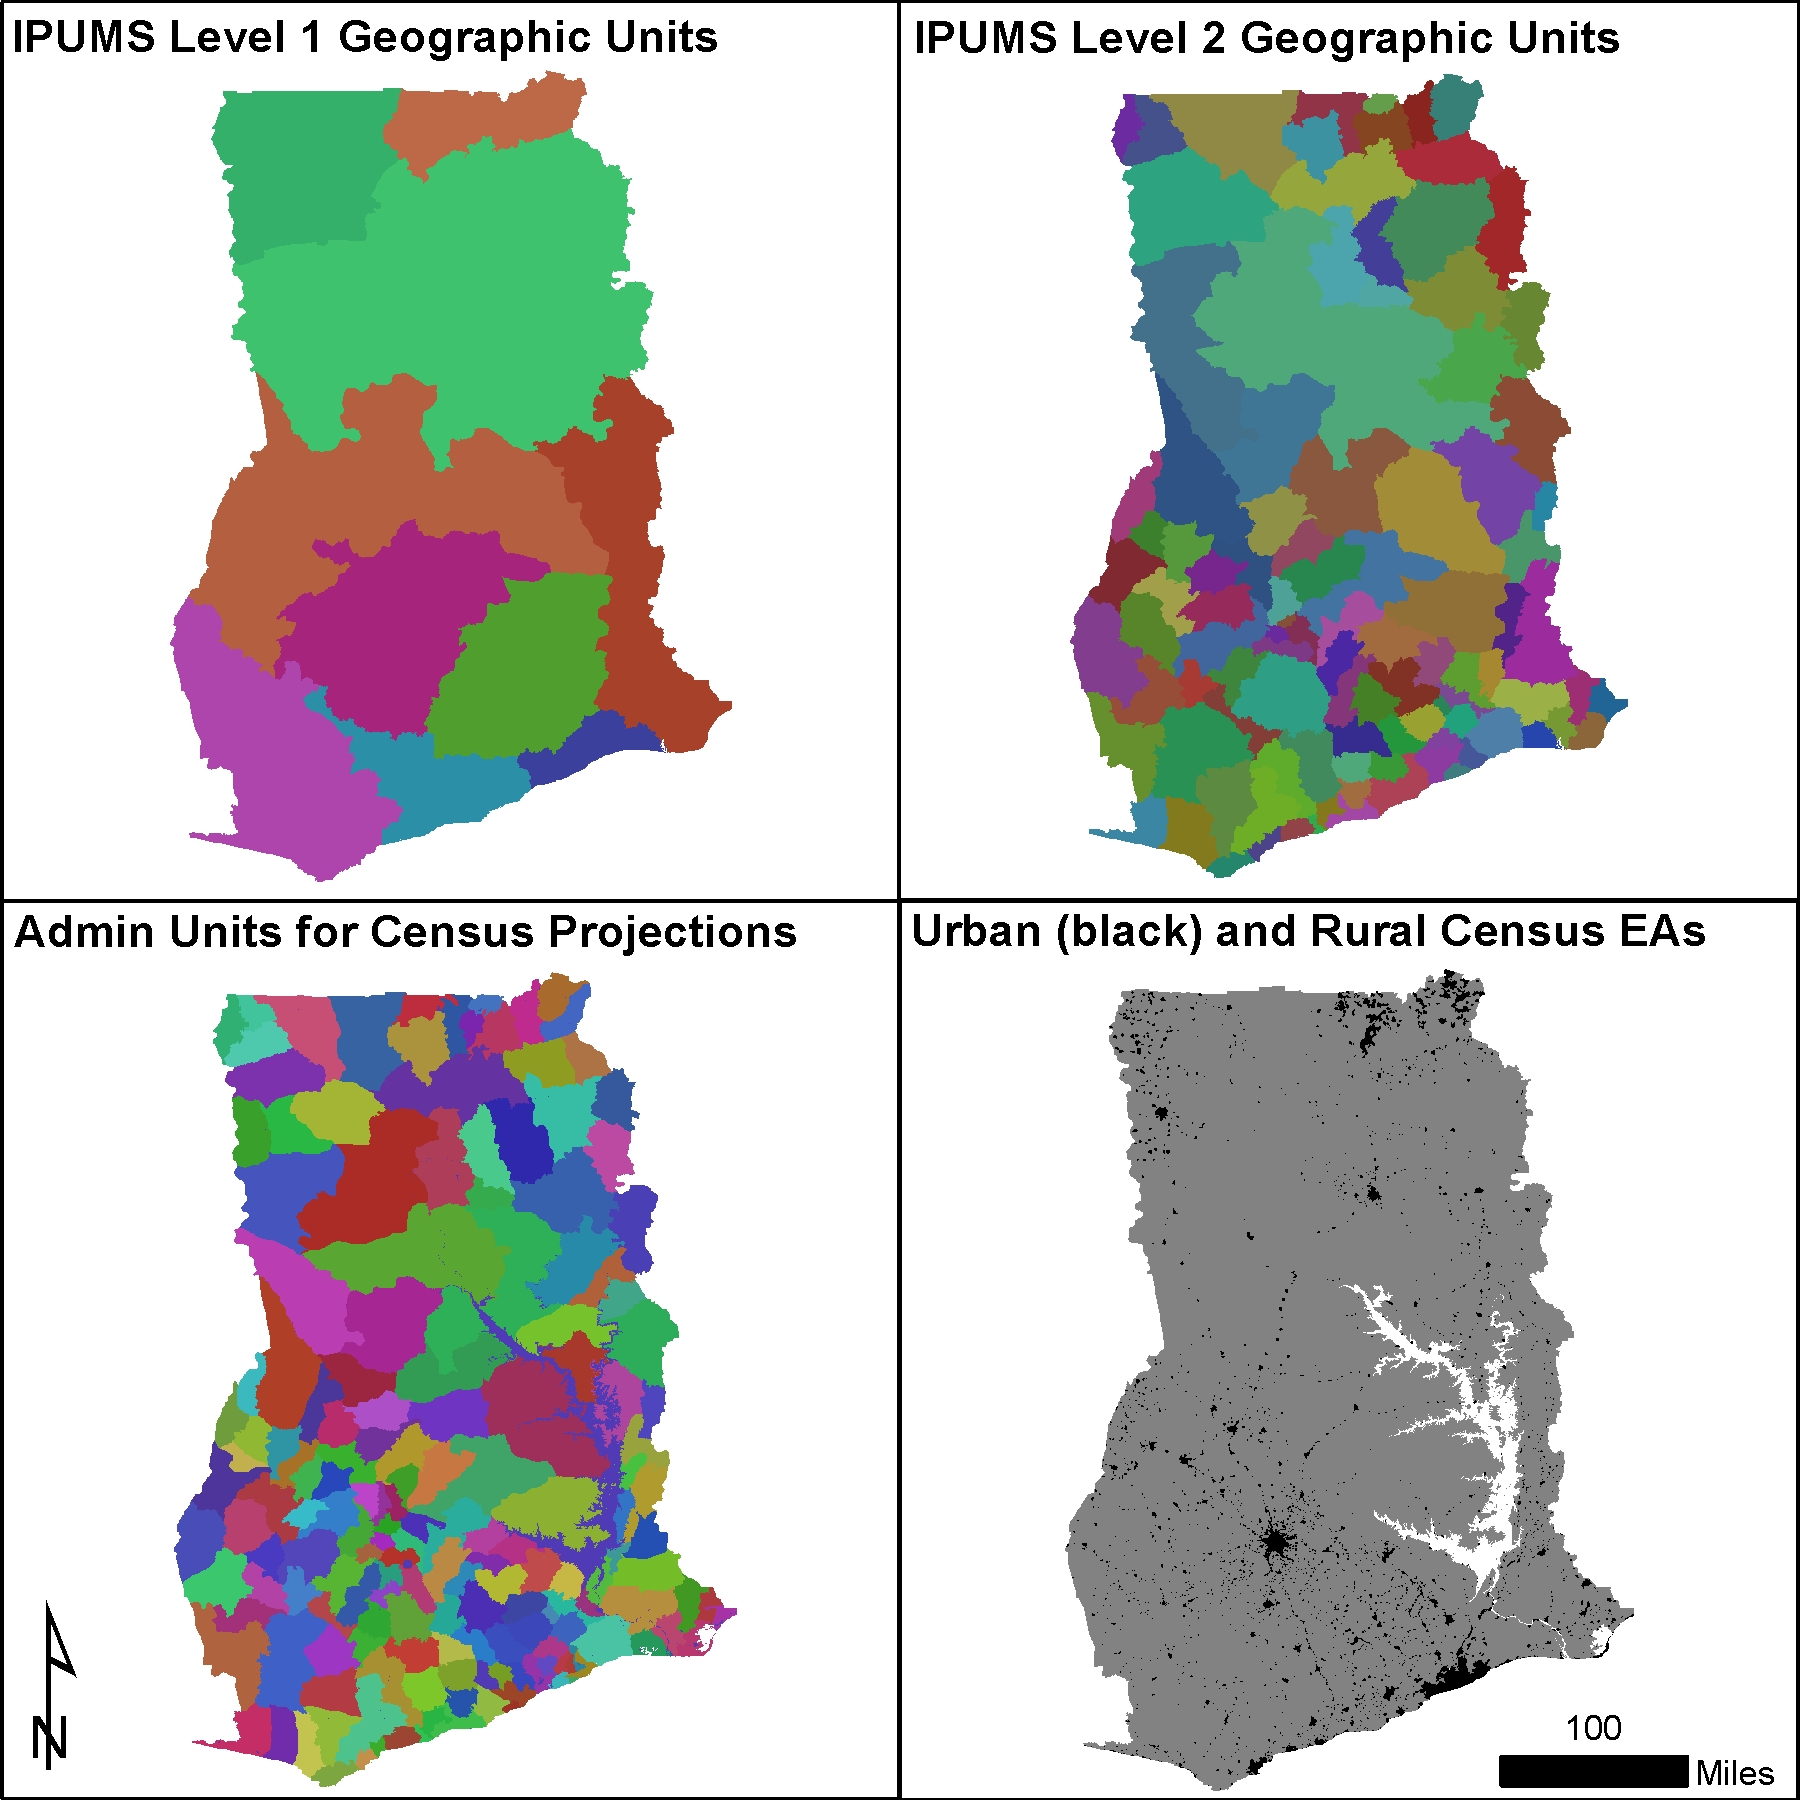
\includegraphics[width=0.6\linewidth]{dat/GHAv1/map} 

}

\caption{Geographic units used for modelling.}\label{fig:map}
\end{figure}

\subsection{Statistical Model}\label{statistical-model}

We developed a Bayesian statistical model to estimate the average number
of \emph{people per housing unit} and the average number of
\emph{housing units per building} from these data.

\subsubsection*{Indexing}\label{indexing}
\addcontentsline{toc}{subsubsection}{Indexing}

The indexing used throughout the model description (below) is as
follows:

\emph{Households (h)} contained within the IPUMS data. There were a
total of 570,234 households from the Ghana census microdata and we used
a representative 70\% sample to fit our model (selected at random using
the SAMPLE attribute of the IPUMS data). The remaining 30\% was used for
out-of-sample model validation.

\emph{Age-sex groups (k)} that included 36 bins: under 1 year, 1 to 5
years, 80+ years, and 5 year intervals in between for both males and
females.

\emph{Settlement type (t)} for each enumeration area from the 2010 Ghana
census. We summarized these as either urban (1) or rural (2).

\emph{Age-sex regions (r)} were defined by the level 1 geographic
boundaries from IPUMS \citep{mpc2019integrated}. We estimated the
proportion of the population in each age-sex group for urban and rural
areas within each of these 10 regions.

\emph{Household geographies (g)} were defined by the level 2 geographic
boundaries from IPUMS \citep{mpc2019integrated}. We estimated people per
household for urban and rural areas within each of these 102
geographies.

\emph{Population units (u)} were defined by the level 3 administrative
boundaries from census projections \citep{worldpop2018globalb}. We
estimated households per building for urban and rural areas within each
of these 170 population units.

\emph{Locations (i)} are 100 meter grid cells that were used for model
predictions.

\subsubsection*{Population Estimates}\label{population-estimates}
\addcontentsline{toc}{subsubsection}{Population Estimates}

To estimate the population for a given location \(i\), we used the
following model:

\begin{equation}
pop_i \sim \textsf{Poisson}(bldg_i \times hpb_{t_i,u_i} \times pph_{t_i, g_i}) \\
pop_{i,k} \sim \textsf{Multinomial}(pop_i, \theta_{t_i,r_i,k})
\label{eq:predict}
\end{equation}

\(pop_i\) is the total population estimated for location \(i\), and
\(pop_{i,k}\) is the number of people within age-sex group \(k\).
\(bldg_i\) is the observed number of building footprints at this
location. \(hpb\) and \(pph\) are estimated parameters measuring
households per building and people per household, respectively. In this
portion of the model, the only observed data are the building counts
\(bldg_i\), settlement type \(t_i\), and the three spatial unit IDs
(\(g_i\), \(u_i\), and \(r_i\)). Note that we are assuming that the
count of building footprints is equivalent to the true count of
buildings.

Estimating the parameters \(hpb_{t,u}\), \(pph_{t,g}\), and
\(\theta_{t,r,k}\) is the focus of the statistical model developed
below.

\subsubsection*{People per Household
(pph)}\label{people-per-household-pph}
\addcontentsline{toc}{subsubsection}{People per Household (pph)}

Single-person households are more common in the Ghana microdata than
could be accounted for by a simple Poison distribution to model
household sizes, so we used a Hurdle model \citep{stan2019stan} to
account for the one-inflated distribution. This involves two processes:

\begin{enumerate}
\def\labelenumi{\arabic{enumi}.}
\item
  \(\alpha_{t,g}\) the probability that a household has only a
  single-person , and
\item
  \(\lambda_{t,g}\) the number of additional people in multi-person
  households other than the head of household.
\end{enumerate}

These two parameters are the basis for estimating people per household
\(pph_{t,g}\) by type and household geographic unit. The Ghana census
microdata (IPUMS 2020) provided the data that we needed to fit this part
of the model. This included a count of people and their ages from a
representative sample of households across the country.

We used a beta-binomial model to estimate the probability of a
single-person household \(\alpha_{t,g}\) in urban and rural settlement
types \(t\) in each geographic area \(g\):

\begin{equation}
single_{t,g} \sim \textsf{Binomial}(hh_{t,g}, \alpha_{t,g}) \\
\alpha_{t,g} \sim \textsf{Beta}(\frac{\bar{\alpha}_{t}}{\tilde{\alpha}}, \frac{1-\bar{\alpha}_{t}}{\tilde{\alpha}})
\label{eq:alpha}
\end{equation}

where \(hh_{t,g}\) is the total number of households surveyed from
settlement type \(t\) in geography \(g\), and \(single_{t,g}\) is the
total number of single-person households surveyed. \(\alpha_{t,g}\) is
the probability that a household contains only a single person.
\(\bar{\alpha}_{t}\) is the mean of \(\alpha_{t,g}\) among geographies
within settlement type \(t\) and \(\tilde{\alpha}\) quantifies variance
among geographies.

We used a Poisson model with LogNormal overdispersion to estimate the
number of people in multi-person households \(\lambda_{t,g}\) (excluding
the head of household):

\begin{equation}
N_h-1 \sim \textsf{Poisson}(\lambda_{h}) T(1,) \\
\lambda_{h} \sim \textsf{LogNormal}(\mu_{t,g}, \sigma_{t,g})
\label{eq:lambda}
\end{equation}

where \(N_h\) is the observed number of people in each multi-person
household \(h\) from the IPUMS census microdata and \(\lambda_{h}\) is
the expected count of household members other than the head of
household. We used \(N_h - 1\) as the response variable so we could use
zero-inflation to account for one-inflated distributions of \(N_h\). The
Poisson distribution is truncated below 1 (notated as T) because the
beta-binomial model (Eq. \eqref{eq:alpha}) already accounts for
single-person households. \(\mu_{t,g}\) is the mean of \(\lambda_h\) (on
the log scale) among households from settlement type \(t\) in geography
\(g\), and \(\sigma_{t,g}\) is the variance (on the log scale) among
households in settlement type \(t\). We modelled \(\mu_{t,g}\) and
\(\sigma_{t,g}\) hierarchically to share information among geographies:

\begin{equation}
\mu_{t,g} \sim \textsf{Normal}(\bar{\mu}_t, \tilde{\mu}) \\
\sigma_{t,g} \sim \textsf{Half-Normal}(\bar{\sigma}_t, \tilde{\sigma})
\label{eq:mu}
\end{equation}

where \(\bar{\mu}_t\) is the mean value of \(\mu_{t,g}\) among
geographies within settlement type \(t\), and \(\tilde{\mu}\) is the
variance among geographies in both settlement types combined. We used
these parameters to estimate a version of \(\lambda\) that was not
constrained by household-level observations:

\begin{equation}
\hat{\lambda}_{t,g} \sim \textsf{LogNormal}(\mu_{t,g}, \sigma_{t,g})
\label{eq:lambdahat}
\end{equation}

When we say that \(\hat{\lambda}_{t,g}\) was not constrained by
household-level observations, we mean that it is constant among
households within a settlement type in a given geography. This is
neccessary to derive the expected values (i.e.~the means) of people per
household to use for population predictions:

\begin{equation}
E(pph_{t,g}) = 1 + (1 - \alpha_{t,g}) \hat{\lambda}_{t,g}
\end{equation}

The priors that we used for parameters in this part of the model were:

\begin{equation}
\bar{\alpha_t} \sim \textsf{Uniform}(0, 1) \\ 
\tilde{\alpha} \sim \textsf{Uniform}(0, 1) \\
\bar{\mu_t} \sim \textsf{Normal}(0, 5) \\ 
\tilde{\mu} \sim \textsf{Uniform}(0, 5) \\ 
\bar{\sigma}_t \sim \textsf{Uniform}(0, 5) \\
\tilde{\sigma} \sim \textsf{Uniform}(0, 5) \\
\end{equation}

Our aim was to use relatively uninformative priors that provided
information about the range of possible values but were not influential
on parameter estimates relative to the data.

Just for comparison purposes, another way to write the Hurdle model from
Eqs. \eqref{eq:alpha} and \eqref{eq:lambda} is:

\begin{equation}
p(N_h - 1 \mid \alpha_{t,g}, \lambda_h)
=
\begin{cases}
\alpha_{t,g} &\quad \text{if } N_h - 1 = 0, \text{ and} \\
(1 - \alpha_{t,g})
   \frac{\displaystyle \textsf{Poisson}(N_h - 1 \mid \lambda_h)}
        {\displaystyle  1 - \textsf{PoissonCDF}(0 \mid \lambda_h)}
&\quad\text{if } N_h - 1 > 0,
\end{cases}
\end{equation}

See the
\href{https://mc-stan.org/docs/2_23/stan-users-guide/zero-inflated-section.html}{Stan
User's Guide} \citep{stan2019stan} for more details about the Hurdle
model specification.

\subsubsection*{Demographic Groups}\label{demographic-groups}
\addcontentsline{toc}{subsubsection}{Demographic Groups}

We used a multinomial-Dirichlet model to account for demographic
structure in the population:

\begin{equation}
M_{t,r,k} \sim \textsf{Multinomial}(\dot{M}_{t,r}, \theta_{t,r,k}) \\
\theta_{t,r,k} \sim \textsf{Dirichlet}(rep(1, K))
\end{equation}

where \(\dot{M}_{t,r}\) is the total number of survey respondents from
our IPUMS sample in settlement type \(t\) within region \(r\), and
\(M_{t,r,k}\) is the number of respondents within age-sex group \(k\)
observed in the census microdata. In this model, the age-sex structure
\(\theta_{t,r,k}\) (i.e.~proportion of population in each group) is a
parameter that is estimated independently for each region and settlement
type. The Dirichlet prior is an uninformative flat prior. \(K\) is the
total number of age-sex groups (i.e. \(K = 36\)). The Dirichlet
distribution produces a vector of probabilities (i.e.~one for each
age-sex group) that must sum to one (i.e.~to represent the total
population).

\subsubsection*{Households per Building
(hpb)}\label{households-per-building-hpb}
\addcontentsline{toc}{subsubsection}{Households per Building (hpb)}

For each population unit \(u\) we know the total count of buildings and
the estimated total population from census projections. From the
previous model components we also have an estimate of the average number
of people per household for household geographies \(g\) and settlement
types \(t\) within the population unit. Our goal now is to use these
pieces of information to estimate the average number of housing units
per building for urban and rural areas within each population unit
\(u\). We accomplished this using the following model:

\begin{equation}
\dot{N}_u \sim \textsf{LogNormal}(log(\bar{N}_u), \tilde{N}_u) \\
\bar{N}_u = \sum_{t=1}^{T} \sum_{g=1}^{G} (B_{t,u,g} \times hpb_{t,u} \times pph_{t,g})
\label{eq:poptotal}
\end{equation}

where \(\dot{N}_u\) are the estimated total population sizes for unit
\(u\) that were provided as input data from census projections
\citep{worldpop2018globala}. \(B_{t,u,g}\) is the observed number of
building footprints within the intersection of geography \(g\),
population unit \(u\), and settlement type \(t\). We modelled
\(hpb_{t,u}\) hierarchically using a log-normal distribution to share
information among population units:

\begin{equation}
hpb_{t,u} \sim \textsf{LogNormal}(\bar{hpb}_{t}, \tilde{hpb})
\end{equation}

where \(\bar{hpb}_{t}\) is the mean of \(hpb_{t,u}\) among population
units within settlement type \(t\), and \(\tilde{hpb}\) is the variance
among population units including both settlement types. These variance
terms did not differ significantly among settlement types, so estimating
a single variance parameter produced similar results to estimating them
seperately.

\subsubsection*{Measurement Error in Census
Projections}\label{measurement-error-in-census-projections}
\addcontentsline{toc}{subsubsection}{Measurement Error in Census
Projections}

We treated the parameter \(\tilde{N}_u\) from Eq. \eqref{eq:poptotal} as
measurement error in the projected census totals \(\dot{N}_u\) that were
used as input data. We provided estimates of measurement error as an
informative prior:

\begin{equation}
\tilde{N}_u \sim \textsf{LogNormal}(log(0.15), 0.5)
\end{equation}

Because we did not have information about the uncertainty of the census
projections, we designed this prior to be as vague as possible while
still resulting in model convergence. The mean of log(0.15) represents
our prior belief that the projected census totals were within about 25\%
of the true population totals, on average across population units \(u\).
The standard deviation of 0.5 represents our prior belief that there may
have been significantly more measurement error in some population units
(e.g.~100\% or more). Because the model is estimating this parameter for
every population unit, the model has the freedom to identify which units
have more or less measurement error, based on information from the rest
of the model.

\subsection{Model Implementation and
Diagnostics}\label{model-implementation-and-diagnostics}

We implemented this Bayesian model using the R statistical programming
language \citep{r2020r} and the rstan package \citep{stan2020rstan}. The
model code and input data are provided as supplementary files that are
described in Appendix A. Convergence of MCMC chains (i.e.~Markov chain
Monte Carlo) was evaluated using the
\href{https://mc-stan.org/rstan/reference/Rhat.html}{Rhat} metric from
the Stan software \citep[\citet{stan2020rstan}]{stan2019stan}. We used
four MCMC chains with a warmup period of 250 iterations followed by a
sampling period of 2500 MCMC iterations per chain.

We have three types of population data that we can use to evaluate model
fit: people per household and people per age-sex group from the
household-level census microdata \citep{mpc2019integrated} and estimates
of total population per region from projected census totals
\citep{worldpop2018globalb}.

In general, we assessed model fit using model residuals
\texttt{(observed\ -\ predicted)} to calculate bias
\texttt{mean(residuals)}, imprecision \texttt{sd(residuals)}, inaccuracy
\texttt{mean(abs(residuals))}, and r-squared percent variance explained
(squared Pearson correlation coefficient). The mean values from
posterior predictions were used for these assessments. We assessed the
model's prediction intervals by calculating the proportion of
out-of-sample observations that were within the prediction intervals. If
the prediction intervals were robust, we expected about 95\% of
out-of-sample observations to fall inside the 95\% prediction intervals
and 50\% of observations fall inside of 50\% prediction intervals.

We assessed model fit at the household-level using the 30\%
out-of-sample subset from the census microdata
\citep{mpc2019integrated}. We analyzed residuals for the following
parameters:

\begin{itemize}
\tightlist
\item
  \(\alpha_{t,g}\) probability of a single-person household,
\item
  \(\lambda_{t,g}\) additional household members in multi-person
  households,
\item
  \(pph_{t,g}\) number of people per household,
\item
  \(\theta_{t,r,k}\) proportion of the population in each age-sex group,
  and
\item
  \(\dot{N}_u\) total population per population unit \(u\).
\end{itemize}

We assessed model fit at the region-level using in-sample data from the
projected census totals \citep{worldpop2018globala}. We generated a
posterior predictions for the total population in unit \(u\) as:

\begin{equation}
\hat{\dot{N}}_u \sim \textsf{LogNormal}(\bar{N}_u, \tilde{N}_u)
\end{equation}

Spatial units \(u\) where there was a large difference between the
modelled population total \(\hat{\dot{N}}\) and the projected census
totals \(\dot{N}\) likely indicates that census projections were
inaccurate in those units, but it could also indicate a lack of model
fit for that location (i.e.~biased estimates of \(hpb_{t,u}\) or
\(pph_{t,g}\)).

\section{Results}\label{results}

The model reached full convergence for all parameters based on the Rhat
metric used by Stan and there were no additional warnings about
instabilities of means, medians, or tails of posteriors.

Full model results can be downloaded from the
\href{https://wopr.worldpop.org/?GHA/Population/v1.0}{WorldPop Open
Population Repository} \citep{leasure2020bayesian}. This included 100 m
gridded estimates with national coverage for:

\begin{enumerate}
\def\labelenumi{\arabic{enumi}.}
\tightlist
\item
  The number of people,
\item
  The number of people in each age-sex group,
\item
  The number of households,
\item
  The average number of people per household,
\item
  The average number of households per building footprint, and
\item
  The average number of people per building footprint.
\end{enumerate}

Posterior estimates for total number of people and people per age-sex
group can be explored on an interactive map using the
\href{https://github.com/wpgp/wopr}{wopr R package} and the
\href{https://apps.worldpop.org/woprVision}{woprVision web application}
(Fig. \ref{fig:woprVision}) \citep{leasure2020wopr}. It is not possible
to validate the model predictions at the 100 m grid cell level because
we do not have geolocated population data. The posterior predictions
have wide confidence intervals that accurately reflect this uncertainty.

\begin{figure}

{\centering 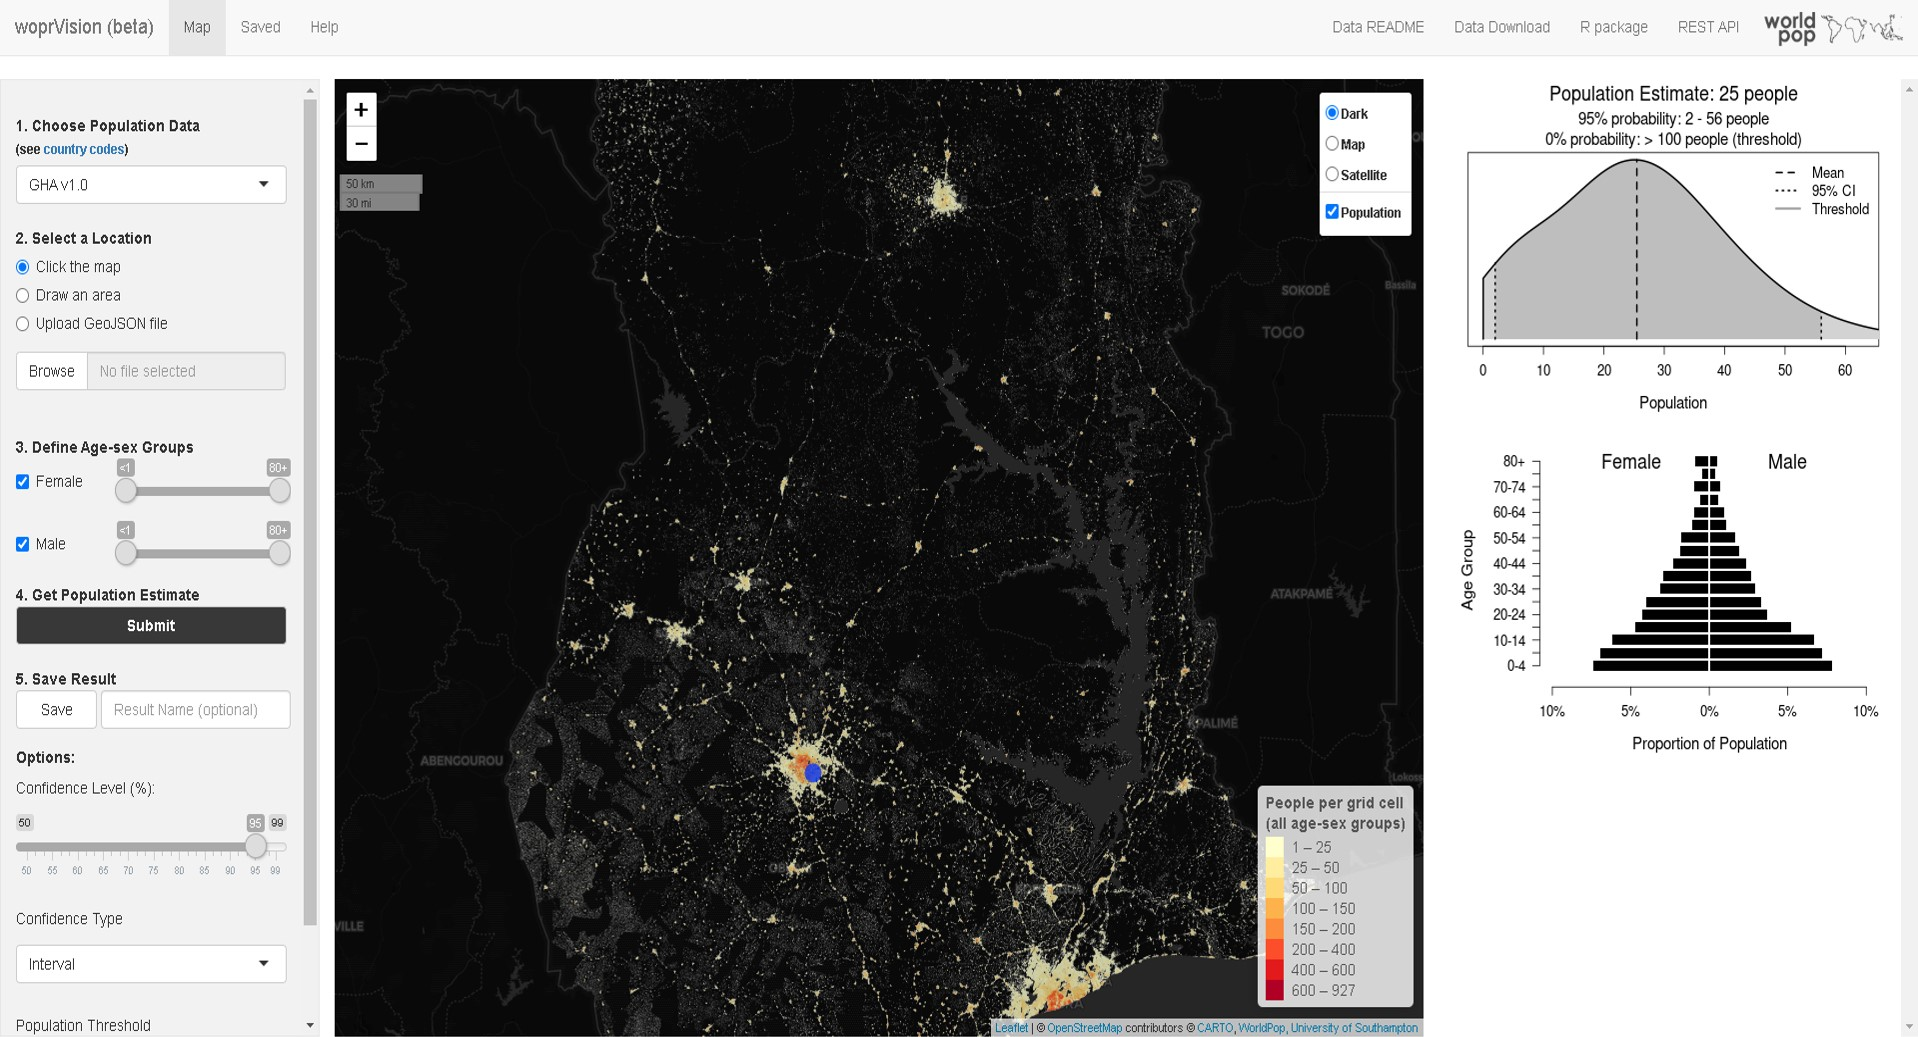
\includegraphics[width=1\linewidth]{dat/GHAv1/woprVision} 

}

\caption{woprVision web application providing access to posterior predictions on an interactive web map (https://apps.worldpop.org/woprVision; select data 'GHA v1.0').}\label{fig:woprVision}
\end{figure}

\subsection{People per household}\label{people-per-household}

Analysis of residuals indicated that estimates of people per household
were relatively unbiased (-6.4\%) but predictoins were very imprecise
(76\%) for individual households (r-squared = 0.05). This was expected
due to the lack of location information from the household data. Despite
imprecise household-specific predictions, the overall distributions of
predicted household sizes were representative of household sizes within
geographic units and settlement types (Fig. \ref{fig:pph}). The
prediction intervals for people per household were robust with 96.8\% of
out-of-sample data falling within the 95\% prediction interval and 69\%
falling within the 50\% prediction interval.

\begin{figure}
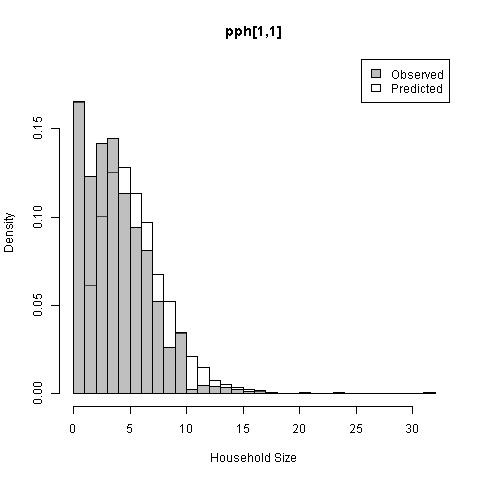
\includegraphics[width=0.5\linewidth]{dat/GHAv1/N/Nhat_1_1} 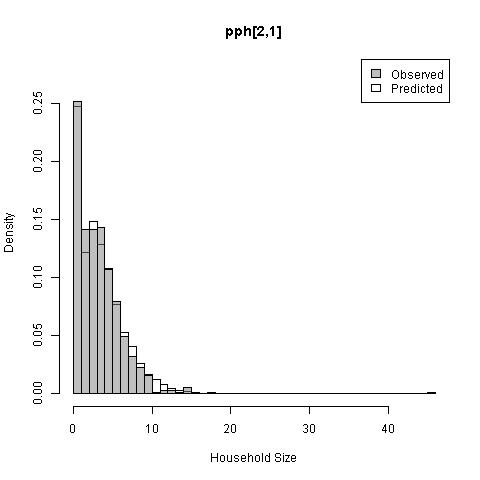
\includegraphics[width=0.5\linewidth]{dat/GHAv1/N/Nhat_2_1} \caption{Distribution of people per household in geographic unit  no. 1 for urban areas (left; t=1, g=1) and rural areas (right; t=2, g=1).}\label{fig:pph}
\end{figure}

Estimates of \(\alpha_{t,g}\) (bias = 1.3\%, imprecision = 19.2\%) and
\(\lambda_{t,g}\) (bias = -1.3\%, imprecision = 8.3\%) were much more
accurate because they were estimated for larger spatial scales
(geographic units \(g\)) with r-squared values of 0.88 and 0.93,
respectively (Fig. \ref{fig:alphalambda}). Remember that
\(\alpha_{t,g}\) is the probability that a household contains only a
single person and \(\lambda_{t,g}\) is the average number of people in a
household other than the head of household. We did not assess the
coverage of the prediction intervals for each of these parameters
individually because they are component parts of a mixture distribution
representing people per household, which was assessed above.

\begin{figure}
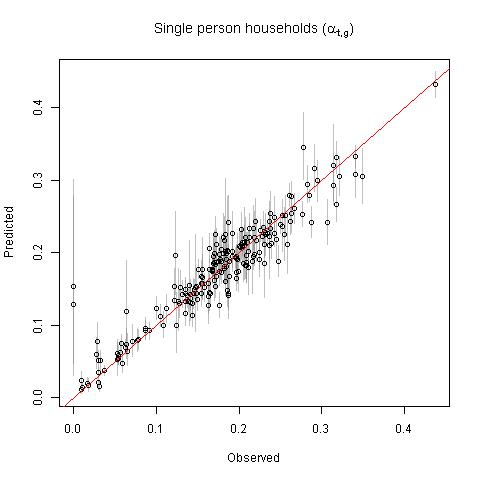
\includegraphics[width=0.5\linewidth]{dat/GHAv1/fit_alpha} 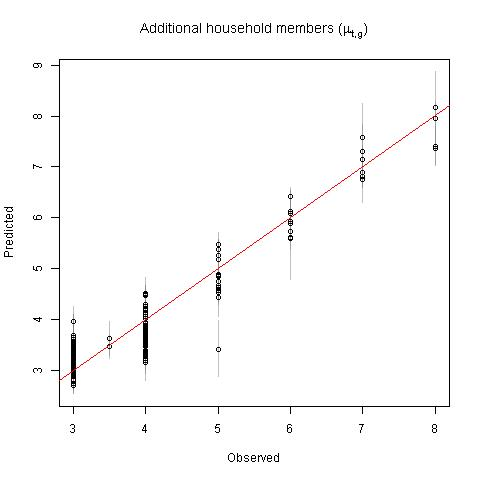
\includegraphics[width=0.5\linewidth]{dat/GHAv1/fit_lambda} \caption{Observed versus predicted parameters for estimating people per household.}\label{fig:alphalambda}
\end{figure}

\subsection{Age-sex structure}\label{age-sex-structure-1}

Estimates of \(\theta_{t,r,k}\) (i.e.~proportion of population in each
age-sex group) had an r-squared of 0.98 compared to out-of-sample data
(Fig. \ref{fig:theta}; bias = -6.6\%, imprecision = 18\%). The slight
negative bias was particularly apparent for estimates of adult males in
some geographic units (see Appendix B). The 95\% prediction intervals
contained only 48\% of out-of-sample data and the 50\% prediction
intervals contained only 21\% of out-of-sample data. The underestimated
prediction intervals may have resulted from the strong constraints of
the Dirichlet distribution requiring the proportions to sum to one.

\begin{figure}

{\centering 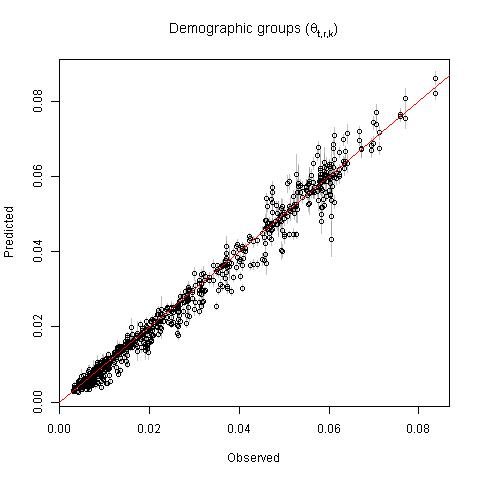
\includegraphics[width=0.5\linewidth]{dat/GHAv1/fit_theta} 

}

\caption{Observed versus predicted proportion of the population in each age-sex group. The plot shows all age-sex groups across all regions.}\label{fig:theta}
\end{figure}

The population pyramids that resulted from the estimates of theta
differed slightly between urban areas and rural areas (Fig.
\ref{fig:pyramid}). Urban areas had a wider base indicating a higher
proportion of children. Within settlement types, there were slight
differences in population pyramids among geographic units (see Appendix
B).

\begin{figure}
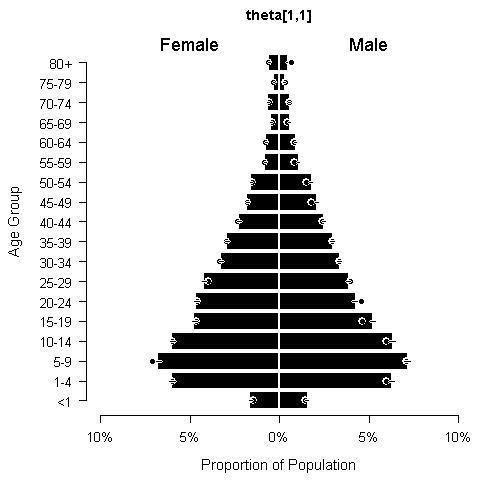
\includegraphics[width=0.5\linewidth]{dat/GHAv1/theta/agesex_1_1} 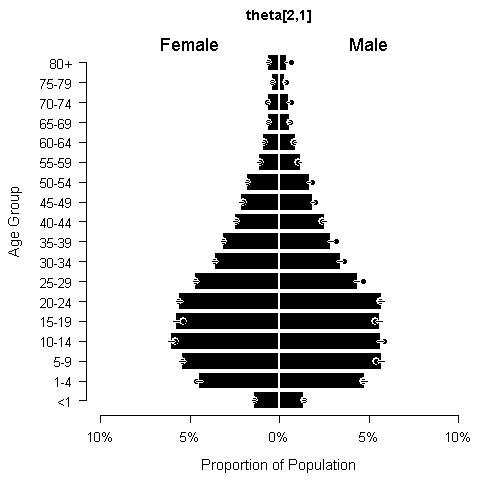
\includegraphics[width=0.5\linewidth]{dat/GHAv1/theta/agesex_2_1} \caption{Population pyramid in region no. 1 for urban areas (left, t=1, r=1) and rural areas (right, t=2, r=1). Dots are observed out-of-sample data, while bars and their credible intervals are posterior predictions from the model.}\label{fig:pyramid}
\end{figure}

Figures comparing model estimates of people per household and age-sex
structure to out-of-sample observations (like Figs. \ref{fig:pph} and
\ref{fig:pyramid}) are provided in Appendix A for all geographic units.

\subsection{Census projections}\label{census-projections}

Model estimates of total population in each population unit \(u\) were
comparable to the projected census totals used as input data for most
areas (r-squared = 0.98), but there were significant divergences in two
units (Fig. \ref{fig:projections}) where the census projections were
likely significant underestimates that did not account for urban growth
into these suburban/rural areas. One of the areas was on the north side
of the city of Kumasi and the other was west of the city of Tamale (see
results at \url{https://apps.worldpop.org/woprVision}; select data ``GHA
v1.0'').

\begin{figure}
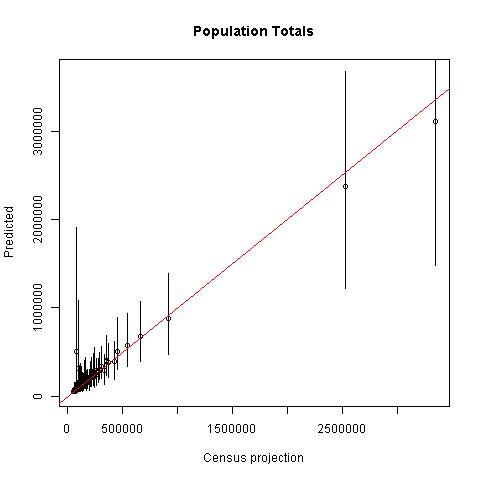
\includegraphics[width=0.5\linewidth]{dat/GHAv1/totpop} 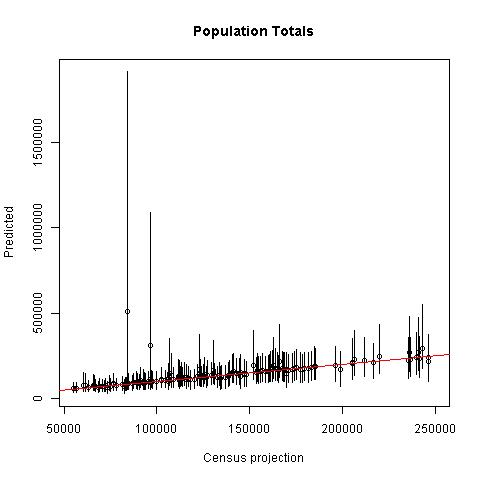
\includegraphics[width=0.5\linewidth]{dat/GHAv1/totpop_zoom} \caption{Census projections versus model predictions of total population sizes in 170 spatial units. The panel on the right is zoomed in to units with less than 250,000 people.}\label{fig:projections}
\end{figure}

\section{Discussion}\label{discussion}

The model is a hybrid between commonly used top-down and bottom-up
approaches \citep{wardrop2018spatially} that are often used to map
populations when complete census results are not available. It is like
bottom-up approaches because it uses household-level survey data that do
not have full coverage of the country. It is like top-down approaches
because it uses projected census totals to constrain population
estimates. Unlike other top-down approaches
\citep{stevens2015disaggregating}, this model enforces a ``soft
constraint'' in which the population totals can deviate significantly
from the census projections provided as input data if the weight of
evidence from the rest of the model suggests the projections are
inaccurate. This approach is unlike top-down and bottom-up approaches
because it cannot use high-resolution geospatial covariates other than
the count of buildings in each 100 m pixel.

This modelling approach produces high resolution gridded population
estimates from publicly available census microdata that have been
standardized across countries by IPUMS International
\citep{mpc2019integrated}. The building footprints that are the other
critical piece of data have been produced for 51 countries in
sub-Saharan Africa \citep{ecopia2020digitize, dooley2020gridded}. This
provides an opportunity to produce rapid population estimates for
countries where both data sets are available. We achieved this by
estimating the average number of \emph{households per building} and the
average number of \emph{people per household} for urban and rural
sub-national geographic units using a hierarchical Bayesian modelling
approach. Importantly, the method accounts for uncertainty which can be
significant for approaches like this that do not have detailed spatial
information associated with the population data, which is the usual
situation when using publicly available data.

This method cannot map variation in people per household or households
per building with precision at the 100 m spatial scale because specific
locations of households are not available for the census microdata. The
model estimates these parameters for urban and rural settlements in over
100 geographic units across the country, but it does not attempt to map
variation within those units. It accounts for that variation as
statistical uncertainty which results in the population estimates having
fairly wide credible intervals. Because we used data from the 2010 Ghana
census to estimate the number of people per household and the proportion
of the population in each age-sex group for urban and rural settlements
in various regions, we have assumed that the patterns of people per
household and age-sex structure have not changed in these areas since
2010. This was a necessary assumption in the absence of more recent
survey data, but the model can be updated when newer data become
available.

We suggest labelling the population estimates as 2018 because this was
the most common satellite image acquisition year (Fig.
\ref{fig:imageryyear}) for imagery used by Maxar Technologies and
Ecopia.AI \citep{ecopia2020digitize} to derive the building footprints.
The year of satellite images varied across the country from 2009 to
2019, depending on the exact location. Refer to the raster
GHA\_buildings\_v1\_1\_imagery\_year.tif \citep{dooley2020gridded} for a
map of the imagery years of building footprints. We assumed that the
building footprints represented all potentially residential buildings.
We did not account for buildings that were missing from the building
footprints or that have since been removed. We did not have quantitative
measures of building footprint accuracy available to us.

\begin{figure}

{\centering 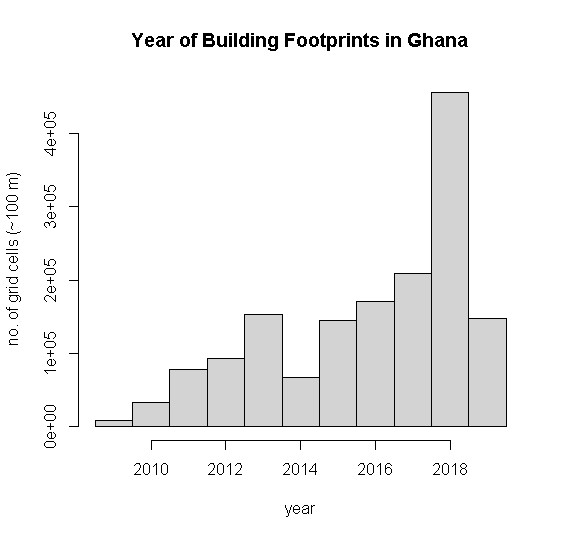
\includegraphics[width=0.5\linewidth]{dat/GHAv1/foot_year} 

}

\caption{Distribution across Ghana of the year of building footprints (Ecopia.AI and Maxar Technologies 2020, Dooley et al. 2020).}\label{fig:imageryyear}
\end{figure}

We identified a few areas for improvement in this model. The credible
intervals for the age-sex structure are not capturing the full range of
variation. One potential solution may be to apply a hierarchical
Dirichlet prior to constrain the population pyramids to share
information among regions. The estimated distributions of people per
household appeared not to fit the out-of-sample data for a few
geographic units and this warrants further investigation, particularly
to understand the effects of outliers on the one-inflated Hurdle model.
It would also be helpful to conduct a formal sensitivity analysis to
assess the influence of the informative prior that we used to quantify
measurement error in the census projections.

In addition to these next steps to improve the method and better
understand its nuances, it will be important to apply it across
countries to understand how generalizable it is. Our intention for this
approach is to apply it rapidly as a gap-filling measure while efforts
are underway to acquire geolocated population data for population
modelling to support development projects, planning for programs, and
census preperations. The model's estimates of people per household and
households per building may also serve as a guide for setting these
parameters in the peanutButter application
\citep{leasure2020peanutbutter} for countries where census microdata or
other household surveys are not publically available.

\section*{Contributing}\label{contributing-6}
\addcontentsline{toc}{section}{Contributing}

This chapter and the methods it describes were developed by Doug Leasure
from the WorldPop Research Group at the University of Southampton with
oversight from Andy Tatem. The work was funded by the Bill and Melinda
Gates Foundation to provide critical spatial data and population
estimates to support polio surveillance and eradication (INV-002697). We
want to acknowledge Vince Seaman from the Bill and Melinda Gates
Foundation and Kebba Touray from the World Health Organization
(AFRO-Polio GIS centre) for facilitating access to data for this
project. We want to thank Edith Darin, Chris Jochem, and Attila Lazar
for thoughtful internal reviews that helped improve the work.

\section*{Suggested Citation}\label{suggested-citation-5}
\addcontentsline{toc}{section}{Suggested Citation}

Leasure DR, Tatem AJ. 2020. A Bayesian approach to produce 100 m gridded
population estimates using census microdata and recent building
footprints. WorldPop, University of Southampton.
{\url{doi:10.5258/SOTON/WP00686}}

\section*{License}\label{license-3}
\addcontentsline{toc}{section}{License}

This chapter may be redistributed following the terms of a
\href{https://creativecommons.org/licenses/by-nd/4.0/}{Creative Commons
Attribution-NoDerivatives 4.0 International (CC BY-ND 4.0) License}.

\section*{Appendices and Supplements}\label{appendices-and-supplements}
\addcontentsline{toc}{section}{Appendices and Supplements}

Appendices and supplementary data for this chapter are available from
Leasure and Tatem \citeyearpar{leasure2020approach} and can also be
downloaded from the WorldPop Open Population Repository (file =
GHA\_population\_v1\_0\_methods.zip).

\chapter{Burkina Faso (v1)}\label{burkina-faso-v1}

Census-based gridded population estimates for Burkina Faso (2019),
version 1.0.

WorldPop, University of Southampton

3 November 2020

\section{Introduction}\label{introduction-2}

In February 2020, the Institut National de la Statistique et de la
Démographie du Burkina Faso (INSD) completed a census exercise aiming at
enumerating the entire country population. Due to security issues in the
North and the East regions, some \emph{communes} (Burkinabe
administrative unit level 3) could be only partially covered by
governmental surveyors (38 out of 351 \emph{communes}). The INSD
requested support from the GRID3 (Geo-Referenced Infrastructure and
Demographic Data for Development) project to estimate the unsurveyed
population.

In November 2020, the INSD released its provisional census population
counts for every \emph{communes} which consisted in estimates for the
unsurveyed areas, and census count corrected via a post-enumeration
survey for the surveyed areas \citep{insd2019recensement}. Parallel to
that traditional publication, the INSD decided to release also a
high-resolution gridded population estimates, and a breakdown by age and
sex group \citep{worldpop2020}.

The purpose of this methodological document is to explain:

\begin{enumerate}
\def\labelenumi{\arabic{enumi}.}
\item
  The bottom-up modelling used to estimate population totals in
  incomplete \emph{communes}
\item
  The top-down modelling used to disaggregate the published census
  population totals \emph{---} a combination of estimation-based and
  enumeration-based \emph{commune} totals \emph{---} into high
  resolution gridded estimates
\end{enumerate}

The produced dataset (WorldPop and Institut National de la Statistique
et de la Démographie du Burkina Faso. 2020) can be downloaded from the
WorldPop Open Population Repository
(\url{https://wopr.worldpop.org/?BFA/Population/v1.0}) and explored on
the woprVision data exploration interface
(\href{https://apps.worldpop.org/woprVision/}{https://apps.worldpop.org/woprVision/).}

\section{\texorpdfstring{Estimating Missed
\emph{Communes}}{Estimating Missed Communes}}\label{estimating-missed-communes}

\subsection{Model Method}\label{model-method}

\begin{figure}

{\centering 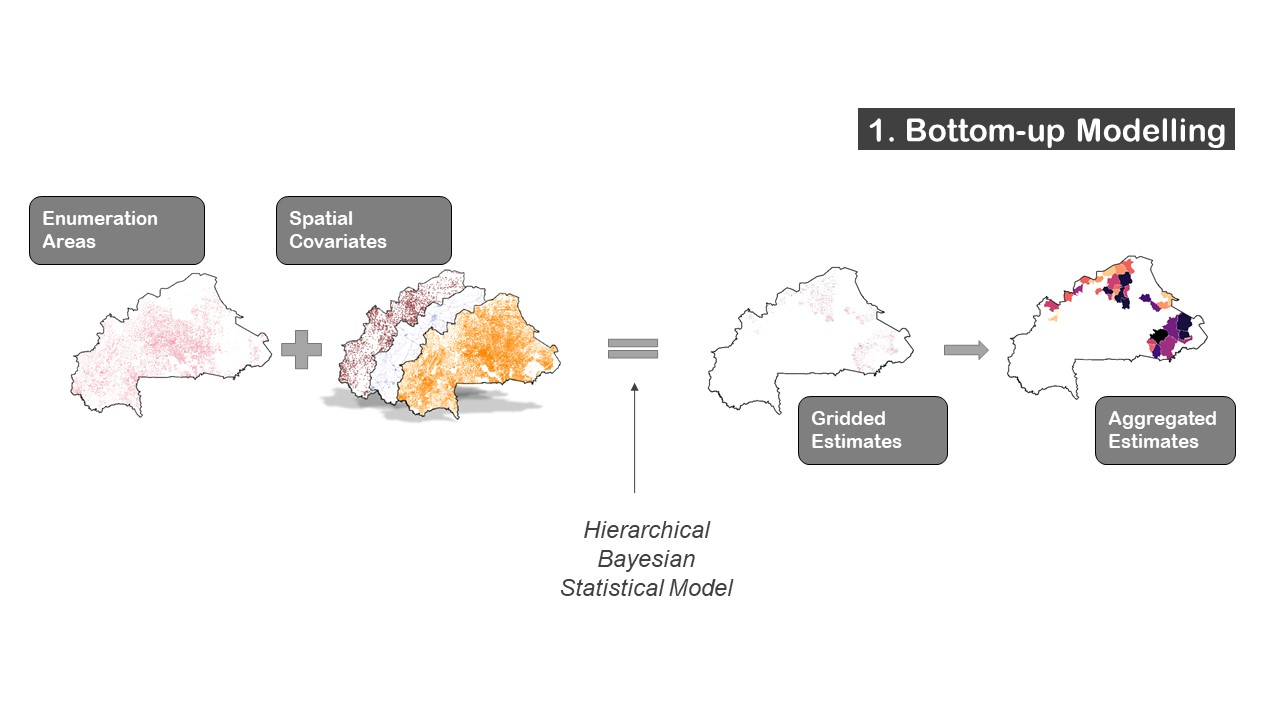
\includegraphics[width=1\linewidth]{dat/BFAv1/schema1_ENG} 

}

\caption{Schema for estimating population in missing communes}\label{fig:schema1}
\end{figure}

The `Bottom-up' modelling followed the hierarchical Bayesian framework
developed by Leasure et al. \citeyearpar{leasure2020national} estimating
population totals using sparse survey data. The method combines
geospatial covariates available for the entire region of study with
observed population data available only for a set of small-size
clusters. The estimated relationship is then applied to the grid cells
(3 arc-seconds, approximately 100m at the equator) of the unsurveyed
areas to predict the population totals. To ensure consistency with the
INSD traditional reporting, the gridded estimates were then aggregated
at the commune level.

The hierarchical probabilistic framework enables to leverage statistical
relationships between population and geospatial covariates from similar
settled locations in order to predict elsewhere and to account for
uncertainty in this process. The following equations describe the
building blocks of the model:

\[
\begin{gathered}
  N_i \sim Poisson( D_i A_i ) \\
  D_i \sim LogNormal( \bar{D}_i, \sigma_{l_1,l_2, l_3}) \\
  \bar{D}_i = \alpha_{l_1,l_2, l_3} + \sum_{k=1}^{K} \beta_k x_{i,k} \\ 
\\
\alpha_{l_1,l_2, l_3} \sim Normal(11,3)\\
\beta_k \sim Normal(0,1)\\
\sigma_{l_1,l_2, l_3} \sim Truncated Normal(0,1,0)
\end{gathered}
\] with:

\begin{itemize}
\tightlist
\item
  a Poisson distribution to model population count \(N_i\) in
  enumeration area \(i\)
\item
  a lognormal distribution to model population density (\(D_i\), which
  is the number of people per settled area in m\(^2\), \(A_i\))
\item
  a hierarchical setting for the variance of the lognormal, \(\sigma\)
  estimated per level \(l_1, l_2\) and \(l_3\)
\item
  a mean of the lognormal, \(\bar{D}\) defined deterministically with a
  hierarchical slope \(\alpha_{l_1,l_2,l_3}\), plus a set of \(K\)
  covariates \(x_k\) with related coefficients \(\beta_k\)
\end{itemize}

\subsection{Model Implementation}\label{model-implementation}

\subsubsection{Input data}\label{input-data-1}

\begin{figure}

{\centering 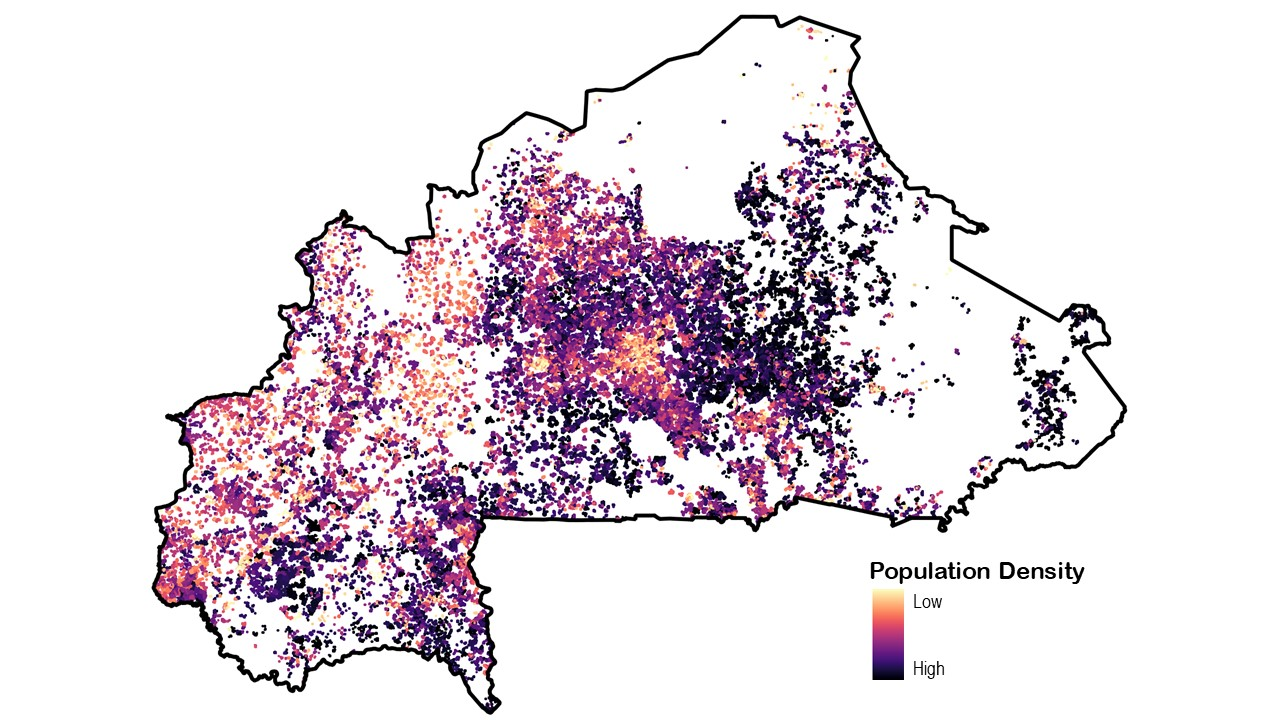
\includegraphics[width=0.8\linewidth]{dat/BFAv1/map_EAs} 

}

\caption{Population density of the selected enumeration areas}\label{fig:map-gps}
\end{figure}

\paragraph{Population}\label{population}

The raw census database consists of the available GPS records for
individual and collective resident households. At the time of the
analysis, digital Enumeration Areas (EA) were not available, thus for
modelling purposes, we compute ad hoc EA boundaries as envelopes around
the GPS points belonging to the same enumeration area. A careful
selection is then made to remove inaccurate EAs due to error in data
collection, EA miss-attribution, imprecise GPS location or inaccurate
GPS recording (due to the location where the surveyor entered the
observation in the device). We implemented the criteria using
quantitative metrics such as: the standard deviation of GPS points for
each EA, the number of observations falling in one grid cell, the
people/building ratio and the people/settled area ratio.

The final database used for modelling contains 15 817 EAs which
represents 69\% of the raw database.

To prevent overestimating population in unsurveyed \emph{communes}, we
removed from every EAs individuals that were recorded as migrants and
originated from the unsurveyed \emph{communes}. This provides us with a
baseline population where displacement from the insecure \emph{communes}
is temporary ignored and tackled at a later stage.

\paragraph{Building footprints}\label{building-footprints}

A core covariate in our model is the building footprints layer provided
by Ecopia.AI and Maxar Technologies \citeyearpar{ecopia.ai2019}. It is a
satellite-imagery-based features extraction at 5m and gives a precise
estimate of the built-up area in Burkina Faso. Figure \ref{fig:img-bf1}
illustrates this for an area in Ouagadougou.

\begin{figure}

{\centering 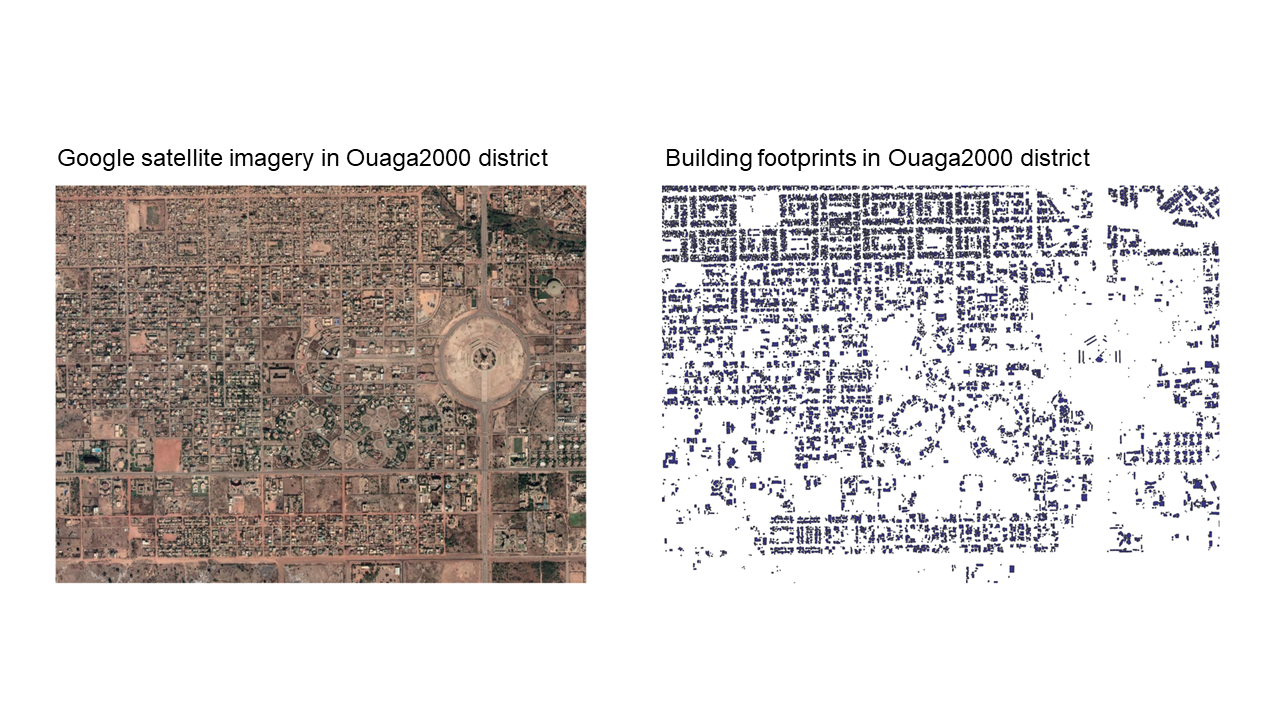
\includegraphics[width=0.8\linewidth]{dat/BFAv1/bf_example} 

}

\caption{Example of the building footprints in Ouagadougou}\label{fig:img-bf1}
\end{figure}

From the building footprints we can calculate the settled area of each
EA (i.e.~the sum of each building area). During the model fitting, this
is used to calculate population densities (people per settled area) from
the observed counts.

The building footprints layer also provides the subset of grid cells for
which to predict population count. We predict population only for the
grid cells considered as settled, that contains at least one building
from the building footprints layer.

\paragraph{Geospatial covariates}\label{geospatial-covariates-1}

To study Burkina Faso spatial population distribution, we selected 5
covariates from different sources based on their assumed correlation to
population densities and on shared range of values between the EA level
dataset and the grid cell level dataset.

The final set of covariates is:

\begin{itemize}
\item
  the count of buildings in a 5km buffer derived from the building
  footprints layer \citep{ecopia.ai2019}
\item
  the distance to temporary rivers and secondary roads provided in the
  Base Nationale de Données Topographiques
  \citep{institutgeographiqueduburkinafaso2015}
\item
  the friction surface used for the Access to Cities project
  \citep{weiss2018}
\item
  the UN-adjusted unconstrained gridded estimates from WorldPop that
  disaggregated the Burkina Faso 2019 census projections
  \citep{worldpop2018global}
\end{itemize}

For classifying settlement consistenly with census definition, we used
the labelling of each EA in the census database as urban or rural to
produce a settlement type prediction at grid cell level.

More precisely, we used the caret R package \citep{kuhn2020} to fit a
Gradient Boosting Machine with two covariates, distance to high urban
settlement \citep{institutgeographiqueduburkinafaso2015} and building
count in a 500m window \citep{ecopia.ai2019}. The area under the curve
metric of the classification model is 0.98, indicating an almost perfect
fit.

\subsection{Model results}\label{model-results}

\subsubsection{Implementing the model}\label{implementing-the-model}

The final models is composed of three nested levels for modelling
population density: the modelled settlement type, the \emph{regions}
(Burkinabe administrative unit level 1) and the \emph{communes}.

Model fit was done using the Stan software \citep{carpenter2017stan}.
Implementing scripts and distribution of estimated parameters can be
found on Github:
\url{https://github.com/wpgp/BFA_population_v1_0_methods/tree/main/supplements}.

To provide population totals for the unsurveyed \emph{communes}, we
aggregated the gridded bottom-up estimates using official boundaries
\citep{institutgeographiqueduburkinafaso2015}. Finally the estimated
population totals were corrected for displacement based on the observed
census migration status data. We added the migrants that were discarded
when processing the census individual database (cf.~Section
\ref{population}) to the \emph{commune} where they were enumerated and
removed them from the unsurveyed \emph{commune} where they were migrated
from.

The model fit and prediction were done in R version 3.5.1., using the
package rstan \citep{stan2020rstan}, sf \citep{pebesma2020}, raster
\citep{hijmans2020}, dplyr \citep{wickham2020}, data.table
\citep{dowle2020} and doParallel \citep{wallig2020}.

\subsubsection{Assessing the model
goodness-of-fit}\label{assessing-the-model-goodness-of-fit}

Prediction power of the final model is first assessed using a training
dataset (70\%) to fit the model and a test dataset (30\%) to estimate
the goodness-of-fit. The correlation between predictions and
observations is 0.8. 95\% of the test observations are in their 95\%
confidence interval. Bias (mean of residuals) is 45 people, imprecision
(standard deviation of residuals) is 263 people and inaccuracy (mean of
absolute residuals) is 169.

\begin{figure}

{\centering 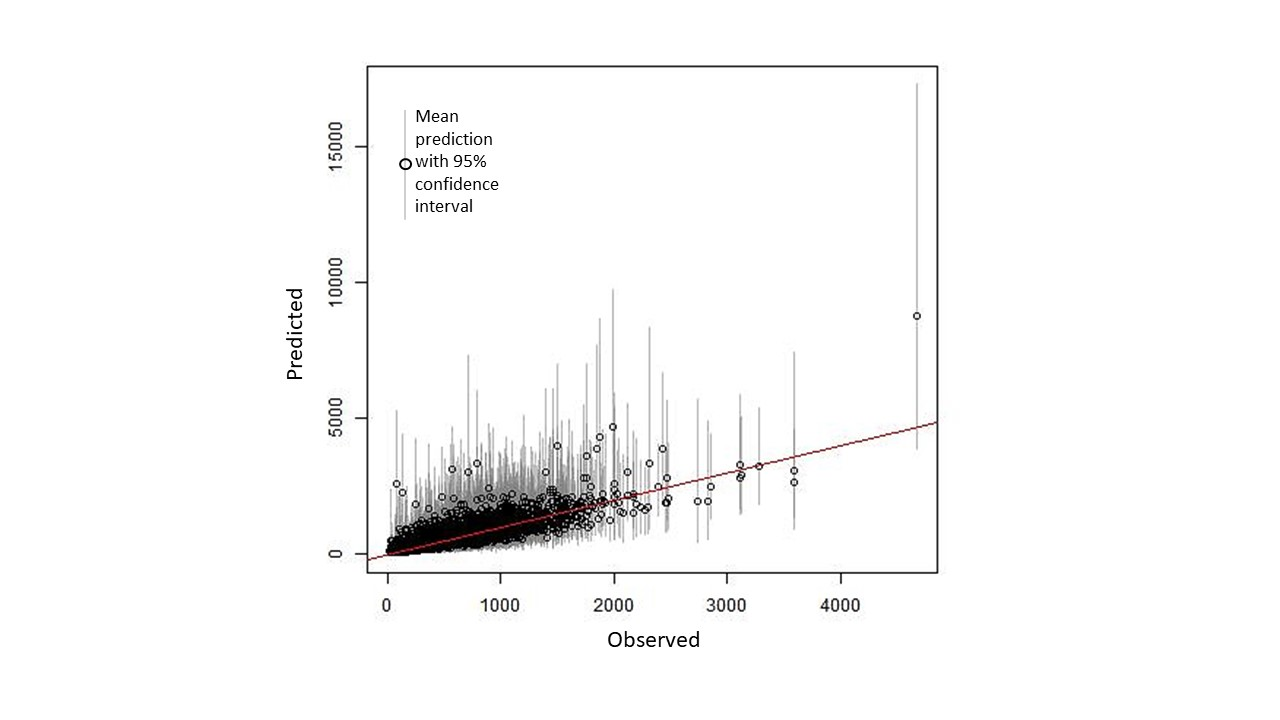
\includegraphics[width=0.8\linewidth]{dat/BFAv1/predictions_scatterplot} 

}

\caption{Scatterplot of observed vs. predicted population count on test EAs. Red line shows perfect prediction}\label{fig:plot-pred}
\end{figure}

The second assessment was undertaken on the population totals for the
completed \emph{communes}, totals that were corrected with omission
rates from the post-enumeration survey. This reference data enables us
to test the sensitivity of the estimates to the selection process, more
precisely two crucial steps:

\begin{enumerate}
\def\labelenumi{\arabic{enumi}.}
\item
  Drawing EA boundaries around GPS points. We have tested two
  alternative scenarios:

  \begin{enumerate}
  \def\labelenumii{\arabic{enumii}.}
  \item
    using a 25m buffer around the GPS points in Ouagadougou, a 25 m
    buffer in Saaba et Bobo-Dioulasso and a 100m buffer in the remaining
    zones;
  \item
    using a 20m buffer around the GPS points in Ouagadougou, a 25m
    buffer in Bobo-Dioulasso and Saaba, a 80m buffer in other urban
    areas and a 120m buffer in rural areas.
  \end{enumerate}
\end{enumerate}

\begin{enumerate}
\def\labelenumi{\arabic{enumi}.}
\setcounter{enumi}{1}
\item
  Selecting the threshold used to discard EA based on the population
  density. We have tested two alternative options:

  \begin{enumerate}
  \def\labelenumii{\arabic{enumii}.}
  \item
    fixed national threshold and
  \item
    custom thresholds based on the maximum population density per admin
    2.
  \end{enumerate}
\end{enumerate}

To assess the predicted totals, we compute a targeted Root Mean Squared
Error for the complete \emph{communes} nested in incomplete
\emph{region}:

\[
\sqrt[][\frac{1}{n} \sum_i (\hat{y}_i - y_i)^2]
\]

where \(n\) is the number of complete \emph{communes} in incomplete
\emph{regions} (\(n\)=141), \(y_i\) the observed census population
totals for \emph{commune} \(i\) and \(\hat{y}_i\) the predicted
population totals for \emph{commune} \(i\).

\begin{Shaded}
\begin{Highlighting}[]
\NormalTok{models <-}\StringTok{ }\KeywordTok{read.csv}\NormalTok{(}\StringTok{"dat/BFAv1/models.csv"}\NormalTok{,  }\DataTypeTok{stringsAsFactors =}\NormalTok{ F, }\DataTypeTok{header=}\NormalTok{F)}
\KeywordTok{colnames}\NormalTok{(models) <-}\StringTok{ }\KeywordTok{c}\NormalTok{(}\StringTok{"Delineation"}\NormalTok{, }\StringTok{"Density Threshold"}\NormalTok{, }\StringTok{"% addditional data discarded"}\NormalTok{, }\StringTok{"RMSE"}\NormalTok{)}
\NormalTok{knitr}\OperatorTok{::}\KeywordTok{kable}\NormalTok{(models, }\DataTypeTok{col.names=}\KeywordTok{c}\NormalTok{(}\StringTok{"Delineation"}\NormalTok{, }\StringTok{"Density threshold"}\NormalTok{, }\StringTok{" "}\NormalTok{, }\StringTok{" "}\NormalTok{), }\DataTypeTok{align =}\StringTok{"l"}\NormalTok{,}\DataTypeTok{escape=}\NormalTok{F, }\DataTypeTok{booktabs=}\NormalTok{T, }\DataTypeTok{caption=}\StringTok{'Sensitivity analysis results on predicted totals'}\NormalTok{) }\OperatorTok\StringTok{ }
\StringTok{    }\NormalTok{kableExtra}\OperatorTok{::}\KeywordTok{add_header_above}\NormalTok{(}\KeywordTok{c}\NormalTok{(}\StringTok{"Selection procedures"}\NormalTok{=}\DecValTok{2}\NormalTok{,}
                     \StringTok{"EA (%)[note]"}\NormalTok{=}\DecValTok{1}\NormalTok{,}
                     \StringTok{"RMSE[note]"}\NormalTok{=}\DecValTok{1}\NormalTok{)) }\OperatorTok\StringTok{ }
\StringTok{  }\NormalTok{kableExtra}\OperatorTok{::}\KeywordTok{add_footnote}\NormalTok{(}\KeywordTok{c}\NormalTok{(}\StringTok{"Additional EAs discarded because of selection procedures (in percentage)"}\NormalTok{, }\StringTok{"RMSE was compiled over the complete communes from incomplete regions"}\NormalTok{), }\DataTypeTok{notation =} \StringTok{"symbol"}\NormalTok{) }\OperatorTok\StringTok{ }
\StringTok{  }\KeywordTok{row_spec}\NormalTok{(}\DecValTok{4}\NormalTok{, }\DataTypeTok{bold=}\NormalTok{T) }\OperatorTok\StringTok{ }
\StringTok{  }\KeywordTok{row_spec}\NormalTok{(}\DecValTok{0}\NormalTok{, }\DataTypeTok{italic =}\NormalTok{ T)}
\end{Highlighting}
\end{Shaded}

\label{tab:unnamed-chunk-14}Sensitivity analysis results on predicted totals

Selection procedures

EA (\%)*

RMSE†

Delineation

Density threshold

Scenario 1

0.16

5

12 163

Scenario 2

0.16

4

10 871

Scenario 2

0.9 x maximum

7

9 966

Scenario 2

0.8 x maximum

9

9 745

* Additional EAs discarded because of selection procedures (in
percentage)

† RMSE was compiled over the complete communes from incomplete regions

Table 1 shows that differentiating the size of the buffer between urban
types does improve the goodness-of-fit. Furthermore choosing a resident
density threshold based on the admin 2 maximum resident density succeeds
in giving a more representative EA dataset that increase the external
goodness-of-fit. Final model is represented in bold.

\clearpage

\section{Estimating Gridded Population for the Entire
Country}\label{estimating-gridded-population-for-the-entire-country}

\subsection{Model Method}\label{model-method-1}

\begin{figure}

{\centering 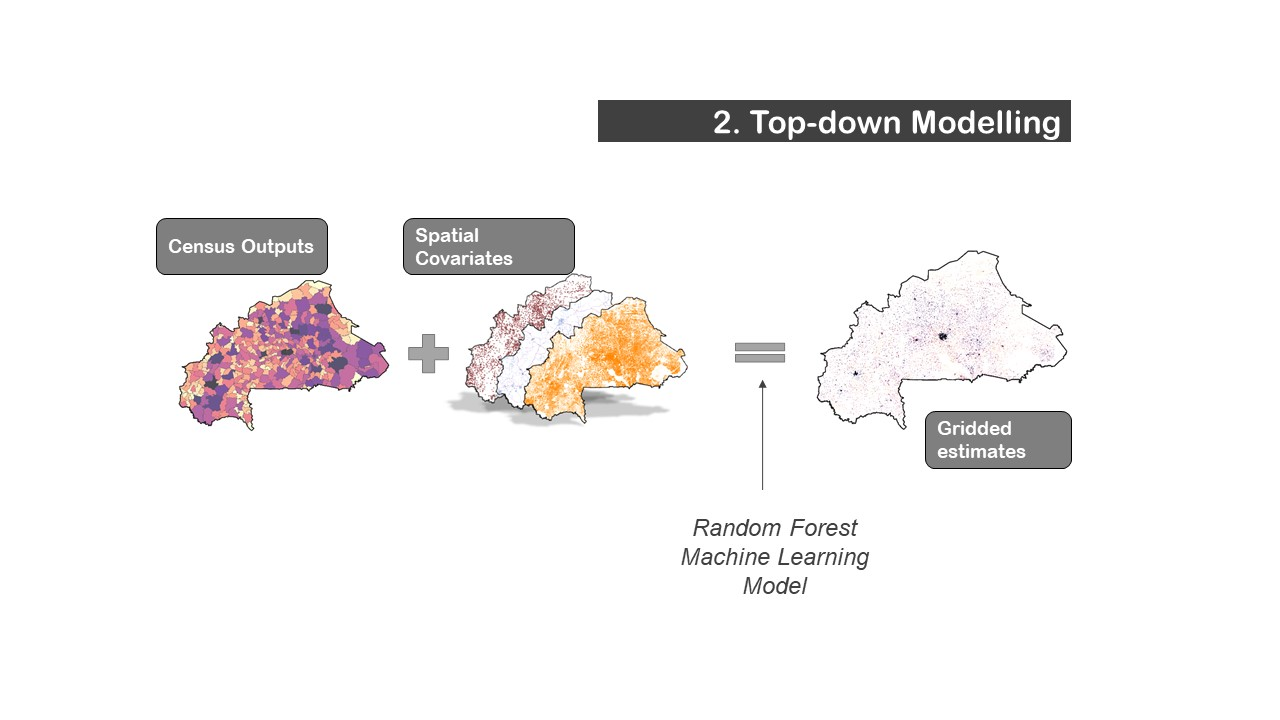
\includegraphics[width=1\linewidth]{dat/BFAv1/schema2_ENG} 

}

\caption{Schema for estimating gridded population for the entire country}\label{fig:schema2}
\end{figure}

To disaggregate the released \emph{communes} census count into
high-resolution gridded estimates, we adapted the dasymetric mapping
explained in Stevens and al. \citeyearpar{stevens2015disaggregating}
using the openly accessible scripts written by Bondarenko and al.
\citeyearpar{bondarenko2018wpgprfpms}. The method consists in modeling
population density by combining geospatial and remotely-sensed data in a
Random Forest framework. This framework is chosen for its great
predictive performance, the absence of complicated tuning parameter and
its robustness to multicolinearity and multi-scale issues in the
predictors \citep{robnik2004improving}.

Once the model is fitted at administrative level, it is then applied to
each grid cell to obtain prediction of population density at a 100m x
100m resolution. This predicted density is then used as a weighting
layer to disaggregate census population counts into the settled pixels
based on a building footprint dataset from Ecopia.AI and Maxar
Technologies \citeyearpar{ecopia.ai2019}. The census counts are thus
unevenly distributed across space to better reflect heterogeneous human
settlement patterns.

\subsection{Model Implementation}\label{model-implementation-1}

\subsubsection{Input data}\label{input-data-2}

\paragraph{Population}\label{population-1}

The officially released population counts at \emph{commune} level,
displayed in Figure \ref{fig:map-pop} combine the surveyed totals
(adjusted with post-enumeration survey non-respondent rates) and the
estimated bottom-up totals.

\begin{figure}

{\centering 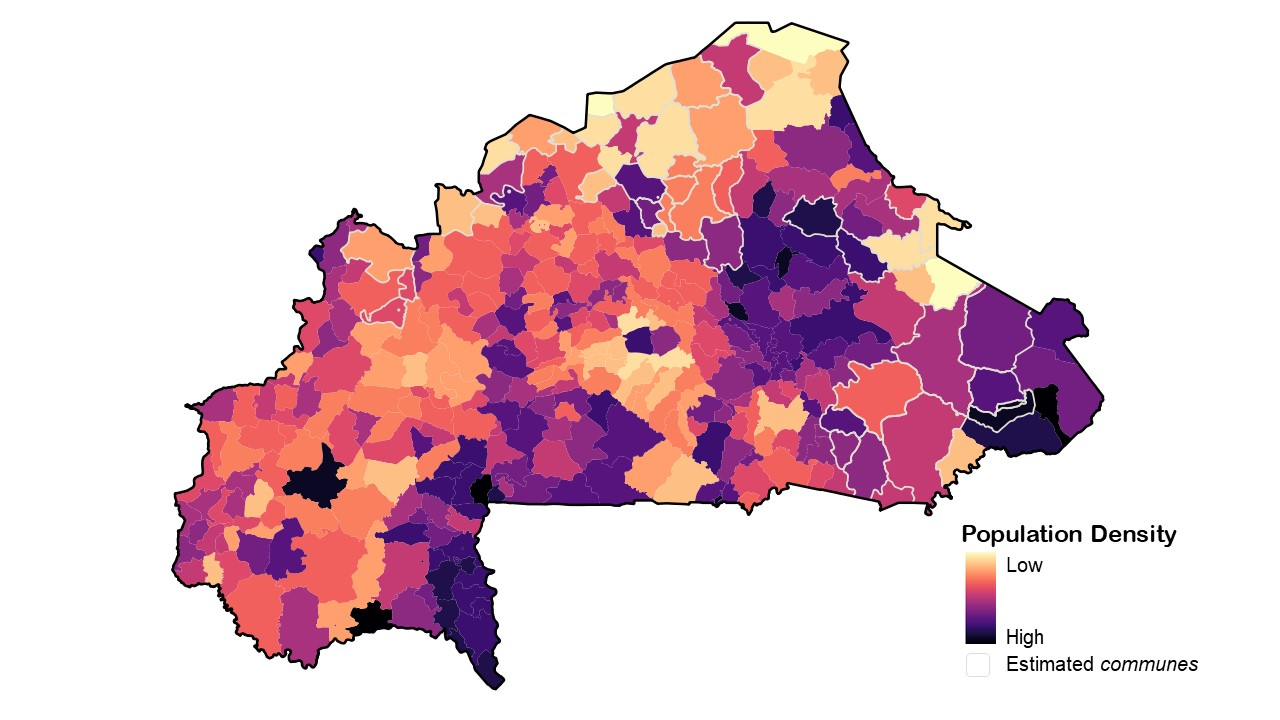
\includegraphics[width=0.9\linewidth]{dat/BFAv1/map_admin3} 

}

\caption{Map of commune population totals}\label{fig:map-pop}
\end{figure}

The census provisional results include also an age and sex decomposition
in 18 five-years-groups at national level \citep{insd2019recensement}.
These will be used to create the age and sex rasters.

\paragraph{Building footprints}\label{building-footprints-1}

The building footprints layer was already presented in Section
\ref{building-footprints}. For the disagregation exercise we derived
four building attributes in addition to building count and settled grid
cells, namely:

\begin{enumerate}
\def\labelenumi{\arabic{enumi}.}
\tightlist
\item
  Building area
\item
  Building perimeter
\item
  Nearest neighbour distance
\item
  Nearest neighbour proximity (1/distance)
\end{enumerate}

The above building attributes are summarised at grid cell level using
eight aggregation methods: mean, median (med), standard deviation (sd),
mean absolute deviation (mad), minimum, maximum, relative standard
deviation (mean/sd) and relative mad (mad/med). Metrics based on the
standard deviation or mean absolute deviation indicate the level of
heterogeneity of the pixel.

Despite the seemingly similarities between some building-footprints
derived covariates, the underlying goal is to increase weak signals for
the Random Forest modelling whose predictions will not be impacted by
high level correlation \citep{genuer2010variable}.

\paragraph{Geospatial covariates}\label{geospatial-covariates-2}

In addition to spatial settlement characteristics (contained in the
building footprints), we use geospatial covariates to explain the
broader context of population distribution.

We constructed 27 additional covariates from six data sources:

\begin{itemize}
\item
  3 from the covariates mapped by the
  \href{https://malariaatlas.org/}{Malaria Atlas Project} for their
  `Accessibility to cities' and `Housing in Africa' projects: travel
  time in 2015, friction surface in 2015 \citep{weiss2018global} and
  mapping of improved housing conditions in 2015
  \citep{tusting2019mapping}.
\item
  4 from the climatic covariates from the
  \href{https://catalogue.ceda.ac.uk/uuid/10d3e3640f004c578403419aac167d82}{Climatic
  Research Unit}: temperature, precipitation, cloud cover and wetness
  \citep{harris2020version}
\item
  9 from the ESACCI
  \href{https://land.copernicus.eu/global/products/lc}{land cover
  classification} \citep{marcel_buchhorn_2020_3939050}, divided in the 9
  overarching classes for which we computed the grid-cell-based distance
\item
  3 from the
  \href{https://academiccommons.columbia.edu/doi/10.7916/d8-h47k-8637}{settlement
  extent} \citep{network_grid3_2020} classified in 3 types (hamlet,
  small settlement, built-up areas) for which we computed the
  grid-cell-based distance
\item
  5 from the Base Nationale de Données Topographiques
  \citep{institutgeographiqueduburkinafaso2015}: the rivers network, the
  roads network and the settlement points classified in three types
  according to their urban status (low, middle, high), for which we
  computed the grid-cell-based distance
\item
  the WorldPop gridded census projection of 2019
  \citep{worldpop2018global}
\end{itemize}

\subsection{Model Results}\label{model-results-1}

\subsubsection{Implementing the model}\label{implementing-the-model-1}

To model the relationship between census data and the entire set of
covariates, we transform the population count into population density by
dividing it with the area of all settled grid cells in the
\emph{commune} and then log-transform it \citep{stevens2015}. We then
average the covariates using zonal mean for every \emph{communes}. The
procedure developed in Bondarenko et al.
\citeyearpar{bondarenko2018wpgprfpms} was used to both tune the Random
Forest model and select covariates using their importance score to speed
up the per-pixel prediction.

Once the model is fitted at \emph{commune} level, we use it to predict
the population density for each grid cell. This predicted density is
then used as a weight to disaggregate the total population count for
each \emph{commune}. The disaggregated gridded population estimates are
multiplied by the age and sex proportions from the national demographic
pyramid to estimate population counts per age and sex group for each
grid cell.

The code for the model fit and prediction can be found on Github:
\url{https://github.com/wpgp/BFA_population_v1_0_methods}

The fit and the prediction were done in R version 3.5.1., using the
package randomForest \citep{cutler2018}, sf\_0.9-5 \citep{pebesma2020},
raster \citep{hijmans2020}, dplyr \citep{wickham2020}, data.table
\citep{dowle2020} and doParallel \citep{wallig2020}.

\subsubsection{Assessing the model
goodness-of-fit}\label{assessing-the-model-goodness-of-fit-1}

\textbf{Covariates importance} We assess the importance of a predictor
by showing the relative increase in the mean square error when the
predictor is removed from the model. The order of magnitude might not be
robust to the collinearity observed in the covariates set but the
relative ranking is \citep{genuer2010variable}.

\begin{figure}

{\centering 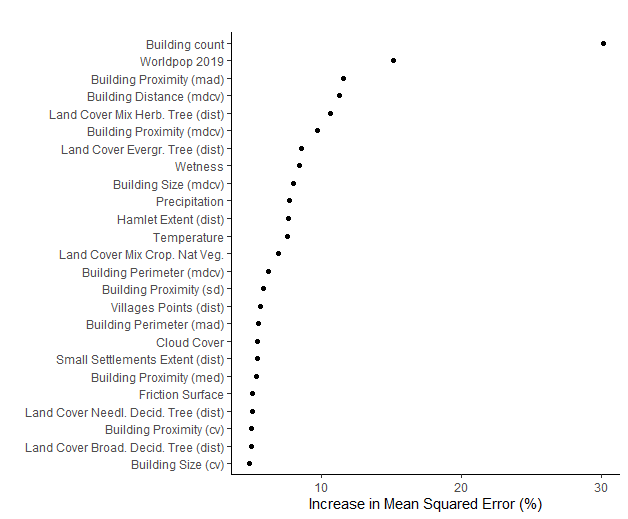
\includegraphics[width=0.6\linewidth]{dat/BFAv1/imp_plot} 

}

\caption{Top 25 Covariates importance in the Random Forest model}\label{fig:imp}
\end{figure}

Figure \ref{fig:imp} shows that the mean building count per pixel is by
far the most important predictor, followed by the gridded population
projections from WorldPop that informs population distribution from
previous censuses. The presence in the top 25 covariates of different
land cover classes confirms previous findings on the predictive power of
land classification \citep{lloyd2019global}.

An interesting additional feature is the strong predictive power of
building-derived metric depicting heterogeneity in a grid cell (standard
deviation -sd-, mean absolute deviation -mad-, coefficient of variation
-cv- and relative mean absolute deviation -mdcv-).

\textbf{Assessing the model} A metric that is commonly used to assess a
Random Forest model is the percentage of variance explained
\citep{liaw2002}. It corresponds to the ``out-of-bag'' mean squared
error divided by the variance of the observations:
\[1 - \frac{\sum_i (y_i - \hat{y}_i)^2}{\sum_i (y_i - \bar{y})^2}\]whre
\(y_i\) is the observed population totals for \emph{commune} \(i\) with
\(\bar{y}\) its corresponding average and \(\hat{y}_i\) is the predicted
population totals for \emph{commune} \(i\) on a test dataset.

In our model the percentage of variance explained is equal to 70.1\%.
For comparison the model developed by Stevens et al.
\citeyearpar{stevens2015disaggregating} for Burkina Faso using census
projections and a standardised set of covariates \citep{lloyd2019global}
had a percentage of variance explained of 59.1\%\footnote{See Burkina
  Faso 2019 in \url{http://dx.doi.org/10.5258/SOTON/WP00645} for more
  details.}.

The difference is explained by the custom set of covariates used in our
model, especially the one derived from the building footprints, and the
restriction of population estimation and prediction to the settled grid
cells.

\textbf{Assessing the prediction} In Stevens and al.
\citeyearpar{stevens2015disaggregating} external validation was
undertaken by applying the modelling process to a coarser census scale
and then aggregating predicted population per pixel at the finer census
unit to compare it with census results. However in Burkina Faso, the
coarser administrative unit after the \emph{commune} is the
\emph{province} level that has only 45 units. We considered this sample
size too small to perform a meaningful model assessment of the Random
Forest modelling.

Nonetheless, we had access to the raw census database where household
GPS points provide a geo-tagging of enumeration areas across the
country. Thus, this offers the possibility to check the model
performance at a fine spatial scale. We manually selected a subset of 50
enumeration areas across the country in different settlement settings
based on the visual assessment of the satellite imagery. We then
computed a predicted population by summing up the corresponding grid
cells and performed a comparison analysis based on the relative
prediction error (Figure 8 and 9):

\[
\frac{\hat{y} - y}{y}*100
\]

where \(\hat{y}\) is the predicted and \(y\) the observed EA population
count.

\begin{figure}

{\centering 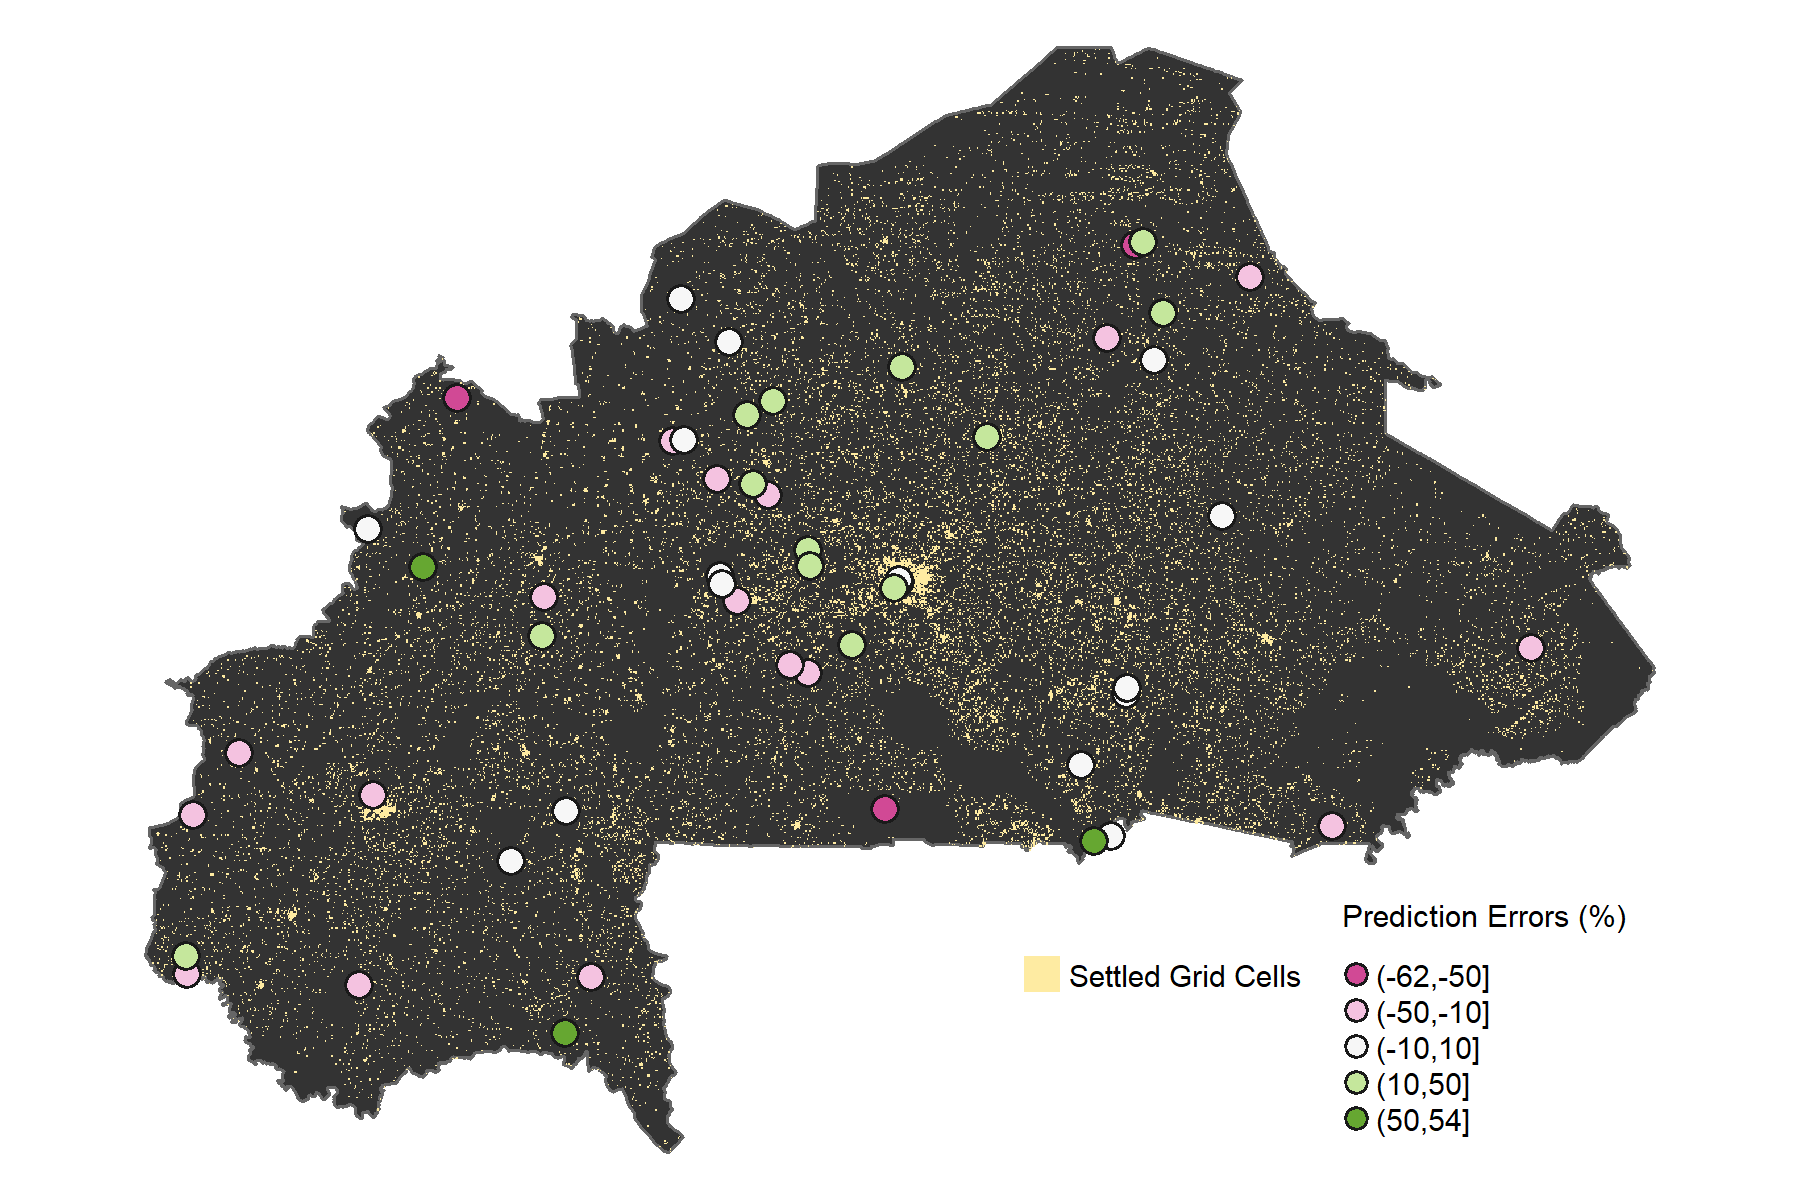
\includegraphics[width=0.8\linewidth]{dat/BFAv1/map-ea-test} 

}

\caption{Spatial distribution of the relative prediction errors. Dots shows the location of the selected EAs. The colours show the ranges of predictive errors. Settled pixels are shown in yellow.}\label{fig:diff}
\end{figure}

\begin{figure}

{\centering 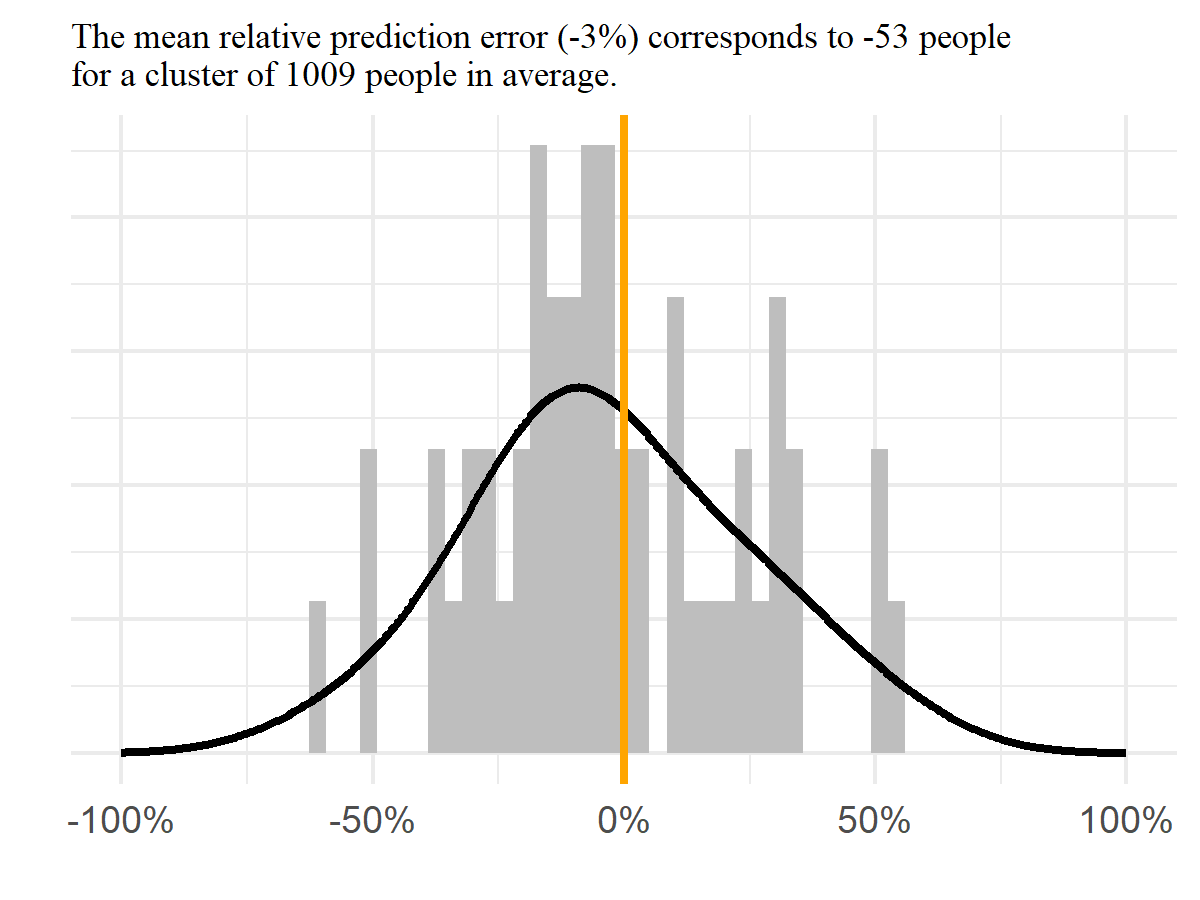
\includegraphics[width=16.67in]{dat/BFAv1/hist-diff} 

}

\caption{Distribution of the relative prediction errors.Grey bars represent each of the 50 selected EAs.The orange line shows the location of the 0\% error, the black line summarises the overall error distribution.}\label{fig:diff2}
\end{figure}

Figure \ref{fig:diff2} shows an average bias of the prediction of -3\%.
Imprecision (std. of relative error) is 27\% and inaccuracy 21\% (mean
of the absolute relative error).

The greater prediction errors are occurring in rural area as shown by
the spatial distribution of the settled cells without clear geographical
clustering (Figure \ref{fig:diff}).

\clearpage

\section{Discussion}\label{discussion-1}

The assumptions and limitations of this study can be summarised by
topics.

\textbf{Country extent} Administrative boundary datasets include the
entire surface of the country. Any settled grid cells outside of the
boundaries from the Base Nationale de Données Topographiques
\citep{institutgeographiqueduburkinafaso2015} were not included.

\textbf{Data date} Although the input data have varying reference years,
the estimates should be considered as representing late 2019 as thisis
the date of the census data collection.

\textbf{Settlement type} The population counts in areas with primarily
non-residential buildings may be over-estimated. Caution should be taken
when using the population data in industrial (and other primarily
non-residential) areas. Furthermore little variation can be modelled for
densely populated urban areas. This is due to the scale of the input
data used to fit the model, namely at administrative level 3, that does
not capture well variation in a dense city such as Ouagadougou.
Therefore precautions shall be taken when focusing the analysis in urban
zones.

\textbf{Building footprints} We assume that the building footprints data
is accurate and that each building polygon corresponds to a building
structure. However the date of the satellite imagery spans from 2009 to
2019 (see Figure \ref{fig:hist-bf}). The estimated population counts may
be inaccurate in areas where the imagery is old and buildings have
recently been constructed. This issue was observed in the towns of
Zorgho, Bâtié and Nanoro. But it is minimized by old satellite imagery
being only used in remote area.

\begin{Shaded}
\begin{Highlighting}[]
\NormalTok{img_date <-}\StringTok{ }\KeywordTok{data.frame}\NormalTok{(}\DataTypeTok{date=}\KeywordTok{c}\NormalTok{(}\StringTok{"<2016"}\NormalTok{, }\DecValTok{2016}\OperatorTok{:}\DecValTok{2019}\NormalTok{), }\DataTypeTok{prop=}\KeywordTok{c}\NormalTok{(}\FloatTok{0.19}\NormalTok{, }\FloatTok{0.07}\NormalTok{, }\FloatTok{0.22}\NormalTok{, }\FloatTok{0.37}\NormalTok{, }\FloatTok{0.15}\NormalTok{))}
\NormalTok{ggplot2}\OperatorTok{::}\KeywordTok{ggplot}\NormalTok{(img_date, ggplot2}\OperatorTok{::}\KeywordTok{aes}\NormalTok{(}\DataTypeTok{x=}\NormalTok{date, }\DataTypeTok{y=}\NormalTok{prop))}\OperatorTok{+}
\StringTok{  }\NormalTok{ggplot2}\OperatorTok{::}\KeywordTok{geom_col}\NormalTok{()}\OperatorTok{+}
\StringTok{  }\NormalTok{ggplot2}\OperatorTok{::}\KeywordTok{theme_bw}\NormalTok{()}\OperatorTok{+}
\StringTok{  }\NormalTok{ggplot2}\OperatorTok{::}\KeywordTok{labs}\NormalTok{(}\DataTypeTok{x=}\StringTok{""}\NormalTok{, }\DataTypeTok{y=}\StringTok{""}\NormalTok{)}\OperatorTok{+}
\StringTok{  }\NormalTok{ggplot2}\OperatorTok{::}\KeywordTok{scale_y_continuous}\NormalTok{(}\DataTypeTok{labels =}\NormalTok{ scales}\OperatorTok{::}\KeywordTok{percent_format}\NormalTok{(}\DataTypeTok{accuracy =} \DecValTok{1}\NormalTok{))}\OperatorTok{+}
\StringTok{  }\NormalTok{ggplot2}\OperatorTok{::}\KeywordTok{theme}\NormalTok{(}\DataTypeTok{axis.text =}\NormalTok{ ggplot2}\OperatorTok{::}\KeywordTok{element_text}\NormalTok{(}\DataTypeTok{size=}\DecValTok{14}\NormalTok{))}
\end{Highlighting}
\end{Shaded}

\begin{figure}

{\centering 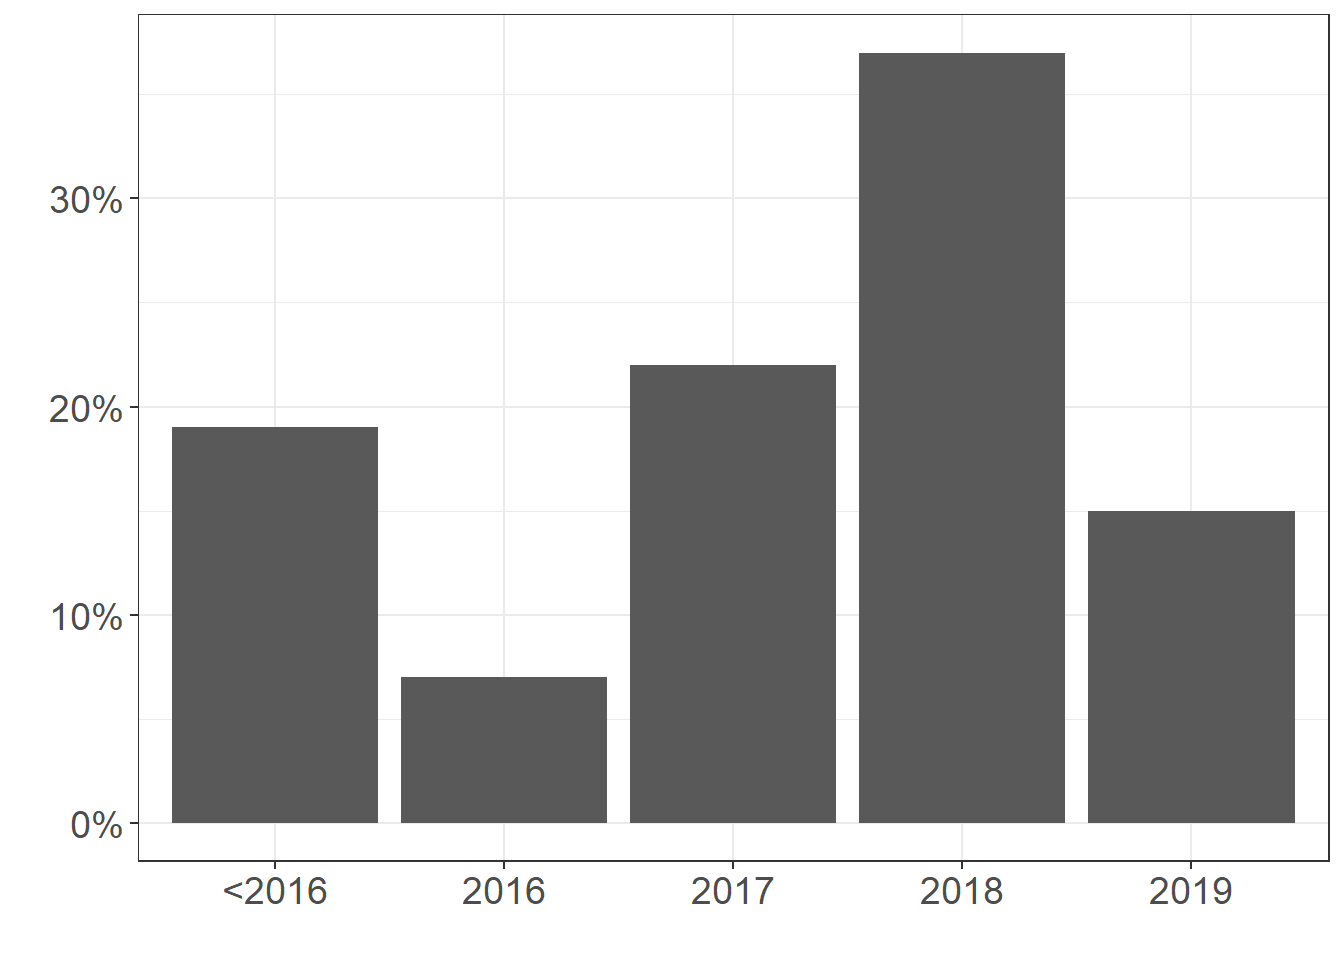
\includegraphics[width=0.4\linewidth]{_main_files/figure-latex/hist-bf-1} 

}

\caption{Satellite imagery date used for extracting building footprints by Ecopia.AI, and Maxar Technologies. (2019)}\label{fig:hist-bf}
\end{figure}

\textbf{Discrete population pattern} Administrative boundaries are
visible in the disagregated estimates whereby sharp population
differences can be found for neighboring grid cells along the
administrative unit delimitation. This is the consequence of the
dasymetric top-down disagregation which ensures that the sum of every
grid cells of the administrative unit does match with the total
provided.

\textbf{Modeled population} The population that is predicted is the
\emph{de jure} resident population as defined by the INSD, that is
\emph{planning in staying or having stayed already six months at the
place where the census is taking place}. This population dataset
represent neither the ambient population, nor captures internal
migration below the \emph{commune} level.

\textbf{Age and sex pyramid} The age and sex proportions are released by
the INSD at the national level, therefore no subnational variations in
proportion were considered for the gridded estimates.

\section*{Contributions}\label{contributions}
\addcontentsline{toc}{section}{Contributions}

This work is part of the GRID3 (Geo-Referenced Infrastructure and
Demographic Data for Development) project funded by the Bill and Melinda
Gates Foundation (BMGF) and the United Kingdom's Department for
International Development (OPP1182408). Project partners include
WorldPop at the University of Southampton, the United Nations Population
Fund (UNFPA), Center for International Earth Science Information Network
(CIESIN) in the Earth Institute at Columbia University, and the
Flowminder Foundation. The Institut National de la Statistique et de la
Démographie supported, facilitated this work, reviewed the results and
provided the census database. The modelling work, geospatial data
processing, stakeholder engagement and model report was led by Edith
Darin with help from Mathias Kuépié. Support for the statistical
modelling was provided by Gianluca Boo, Claire A. Dooley, Douglas R.
Leasure and Chris W. Jochem. Gianluca Boo, Douglas R. Leasure and Attila
N. Lazar provided a thorough review of the manuscript. Oversight was
done by Andrew J. Tatem and Attila N. Lazar.

\section*{License}\label{license-4}
\addcontentsline{toc}{section}{License}

This report may be redistributed using a
\href{https://creativecommons.org/licenses/by-nd/4.0/}{Creative Commons
Attribution-NoDerivatives 4.0 International (CC BY-ND 4.0) License}.

\section*{Suggested Citation}\label{suggested-citation-6}
\addcontentsline{toc}{section}{Suggested Citation}

WorldPop and Institut National de la Statistique et de la Démographie du
Burkina Faso. 2020. Census-based gridded population estimates for
Burkina Faso (2019), version 1.0. WorldPop, University of Southampton.
\url{doi:10.5258/SOTON/WP00687}.

\chapter{Zambia (v1)}\label{zambia-v1}

\begin{quote}
\textbf{Note:} This chapter is currently being drafted. To make
suggestions, please raise an
\href{https://github.com/wpgp/bookworm/issues}{issue} in the bookworm
repository. To make direct edits to the source code, please submit a
\href{https://github.com/wpgp/bookworm/pulls}{pull request} to merge
your code with the ``dev'' branch. Include the tag @cadooley in your
issues or pull requests to notify Claire.
\end{quote}

\begin{quote}
\textbf{Note:} The gridded population estimates for Zambia are available
from the WorldPop Open Population Repository and the woprVision web
application (select ``ZMB v1.0'').
\end{quote}

\section{Introduction}\label{introduction-3}

\section{Methods}\label{methods-1}

\section{Results}\label{results-1}

\section{Discussion}\label{discussion-2}

\section*{Contributing}\label{contributing-7}
\addcontentsline{toc}{section}{Contributing}

This chapter was written by \emph{{[}contributors, please add your name
here{]}}. Funding for the work described in this chapter was provided by
the Bill and Melinda Gates Foundation and the United Kingdom Foreign,
Commonwealth \& Development Office as part of the GRID3 project
(OPP1182408, OPP1182425).

\section*{Suggested Citation}\label{suggested-citation-7}
\addcontentsline{toc}{section}{Suggested Citation}

Doe J, \ldots{} . 2020. Methods to produce bottom-up gridded population
estimates for Zambia, version 1. WorldPop, University of Southampton.
\url{doi:10.5258/SOTON/WP00XXX}

\section*{License}\label{license-5}
\addcontentsline{toc}{section}{License}

This report may be redistributed following the terms of a
\href{https://creativecommons.org/licenses/by-nd/4.0/}{Creative Commons
Attribution-NoDerivatives 4.0 International (CC BY-ND 4.0) License}.

\chapter{Dem. Rep.~of the Congo (v2)}\label{dem.-rep.of-the-congo-v2}

\begin{quote}
\textbf{Note:} This chapter is currently being drafted. To make
suggestions, please raise an
\href{https://github.com/wpgp/bookworm/issues}{issue} in the bookworm
repository. To make direct edits to the source code, please submit a
\href{https://github.com/wpgp/bookworm/pulls}{pull request} to merge
your code with the ``dev'' branch. Include the tag @gianlucaboo in your
issues or pull requests to notify Gianluca.
\end{quote}

\begin{quote}
\textbf{Note:} The gridded population estimates for Democratic Republic
of the Congo are available from the WorldPop Open Population Repository
and the woprVision web application (select ``COD v2.0'').
\end{quote}

\section{Introduction}\label{introduction-4}

\section{Methods}\label{methods-2}

\section{Results}\label{results-2}

\section{Discussion}\label{discussion-3}

\section*{Contributing}\label{contributing-8}
\addcontentsline{toc}{section}{Contributing}

This chapter was written by Gianluca Boo, \emph{{[}contributors, please
add your name here{]}}. Funding for the work described in this chapter
was provided by the Bill and Melinda Gates Foundation and the United
Kingdom Foreign, Commonwealth \& Development Office as part of the GRID3
project (OPP1182408, OPP1182425).

\section*{Suggested Citation}\label{suggested-citation-8}
\addcontentsline{toc}{section}{Suggested Citation}

Boo G, \ldots{} . 2020. Methods to produce bottom-up gridded population
estimates for Democratic Republic of the Congo, version 2. WorldPop,
University of Southampton. \url{doi:10.5258/SOTON/WP00XXX}

\section*{License}\label{license-6}
\addcontentsline{toc}{section}{License}

This report may be redistributed following the terms of a
\href{https://creativecommons.org/licenses/by-nd/4.0/}{Creative Commons
Attribution-NoDerivatives 4.0 International (CC BY-ND 4.0) License}.

\chapter{South Sudan (v2)}\label{south-sudan-v2}

\begin{quote}
\textbf{Note:} This chapter is currently being drafted. To make
suggestions, please raise an
\href{https://github.com/wpgp/bookworm/issues}{issue} in the bookworm
repository. To make direct edits to the source code, please submit a
\href{https://github.com/wpgp/bookworm/pulls}{pull request} to merge
your code with the ``dev'' branch. Include the tag @cadooley in your
issues or pull requests to notify Claire.
\end{quote}

\section{Introduction}\label{introduction-5}

\section{Methods}\label{methods-3}

\section{Results}\label{results-3}

\section{Discussion}\label{discussion-4}

\section*{Contributing}\label{contributing-9}
\addcontentsline{toc}{section}{Contributing}

This chapter was written by Claire A Dooley, \emph{{[}contributors,
please add your name here{]}}. Funding for the work described in this
chapter was provided by the Bill and Melinda Gates Foundation and the
United Kingdom Foreign, Commonwealth \& Development Office as part of
the GRID3 project (OPP1182408, OPP1182425).

\section*{Suggested Citation}\label{suggested-citation-9}
\addcontentsline{toc}{section}{Suggested Citation}

Dooley CA, \ldots{} . 2020. Methods to produce gridded population
estimates accounting for population displacement in South Sudan, version
2. WorldPop, University of Southampton. \url{doi:10.5258/SOTON/WP00XXX}

\section*{License}\label{license-7}
\addcontentsline{toc}{section}{License}

This report may be redistributed following the terms of a
\href{https://creativecommons.org/licenses/by-nd/4.0/}{Creative Commons
Attribution-NoDerivatives 4.0 International (CC BY-ND 4.0) License}.

\chapter*{Population Modelling
Tutorials}\label{population-modelling-tutorials}
\addcontentsline{toc}{chapter}{Population Modelling Tutorials}

This section contains tutorials describing how to implement population
modelling methods using the R statistical programming language.

\chapter*{Resources for Developers}\label{resources-for-developers}
\addcontentsline{toc}{chapter}{Resources for Developers}

\hypertarget{wopr-api}{\chapter{WOPR API}\label{wopr-api}}

The WOPR API provides a way for web servers and other computers to
communicate with the WorldPop Open Population Repository to submit
requests for data and to retrieve results. This can be used to:

\begin{enumerate}
\def\labelenumi{\arabic{enumi}.}
\tightlist
\item
  Automate the process of downloading the latest WorldPop population
  data sets and documentation,
\item
  Submit spatial queries (points or polygons) to the WorldPop server to
  retrieve population estimates within user-defined geographic areas,
\item
  Get estimates of population sizes for specific demographic groups
  (i.e.~age and sex), and
\item
  Get probabilistic estimates of uncertainty for all population
  estimates.
\end{enumerate}

This chapter provides instructions how to utilize each of the following
API endpoints:

\textbf{Data Catalogue}\\
https://wopr.worldpop.org/api/v1.0/data

\textbf{Spatial Queries}\\
https://api.worldpop.org/v1/wopr/pointtotal\\
https://api.worldpop.org/v1/wopr/pointagesex\\
https://api.worldpop.org/v1/wopr/polytotal\\
https://api.worldpop.org/v1/wopr/polyagesex

\textbf{Retrieve Results}\\
https://api.worldpop.org/v1/tasks

\section{Data Download}\label{data-download}

\textbf{API Endpoint:}\\
https://wopr.worldpop.org/api/v1.0/data

This API endpoint will return the WOPR data catalogue in JSON format.

 The JSON is organized with the following hierarchical levels:

\begin{itemize}
\item
  \textbf{country} A three letter code to identify the country that the
  dataset represents. WOPR uses ISO country codes to abbreviate country
  names. For example \texttt{\textquotesingle{}NGA\textquotesingle{}}
  regers to Nigeria.
\item
  \textbf{category} The category describes the types of data available
  for a given country. For example,
  \texttt{\textquotesingle{}Population\textquotesingle{}} refers to
  population estimates.
\item
  \textbf{version} The version of a data release for a given country and
  data type. For example,
  \texttt{\textquotesingle{}v1.2\textquotesingle{}}.
\item
  \textbf{file\_type} The file\_type describes the category of
  individual files. For example,
  \texttt{\textquotesingle{}gridded\textquotesingle{}} refers to gridded
  population estimates, and
  \texttt{\textquotesingle{}sql\textquotesingle{}} refers to the SQL
  database used on the WOPR backend to support the spatial queries
  described below.
\end{itemize}

 Each file has the following attributes:

\begin{itemize}
\item
  \textbf{title} is a short descriptive name of the data set.
\item
  \textbf{desc} is a longer description of the data set.
\item
  \textbf{citation} is the recommended citation.
\item
  \textbf{doi} is the official published DOI (digital object identifier)
  that can be used for citations. The DOI refers to a stable and
  permanent version of the file that is stored at
  ftp://ftp.worldpop.org/repo/wopr. These files may differ slightly from
  the files stored at https://wopr.worldpop.org if minor changes were
  made since the time of the DOI publication.
\item
  \textbf{file} is the file name.
\item
  \textbf{file\_size} is the size of the file on the hard disk (MB).
\item
  \textbf{url} is the URL for downloading the file.
\item
  \textbf{date} is the date the file was released.
\item
  \textbf{hash} is the MD5 hash that can be used to compare files to
  ensure their contents are identical.
\item
  \textbf{git} is the URL for the GitHub repository containing code that
  is relevant to the data set (e.g.~the code used to create the data).
\end{itemize}

\section{Spatial Queries}\label{spatial-queries}

Spatial queries can be submitted to WOPR as points or polygon locations
in a GeoJSON format using several different WOPR API endpoints that will
be described below. Spatial requests are supported for any data releases
in the category \texttt{\textquotesingle{}Population\textquotesingle{}}
that contain an SQL database
\texttt{file\_type=\textquotesingle{}sql\textquotesingle{}} (see Data
Download above).

Before describing the API endpoints, a note about the format of the
results. WOPR will return population estimates for the queried location
and demographic group as a JSON that contains a vector of numbers
representing the population estimate for a given location:
\texttt{122,88,108,119,98,92,98,101,121,103,127,122,103,118,...}. A
histogram of these numbers will graphically illustrate the population
estimate and its uncertainty as a probability distribution:

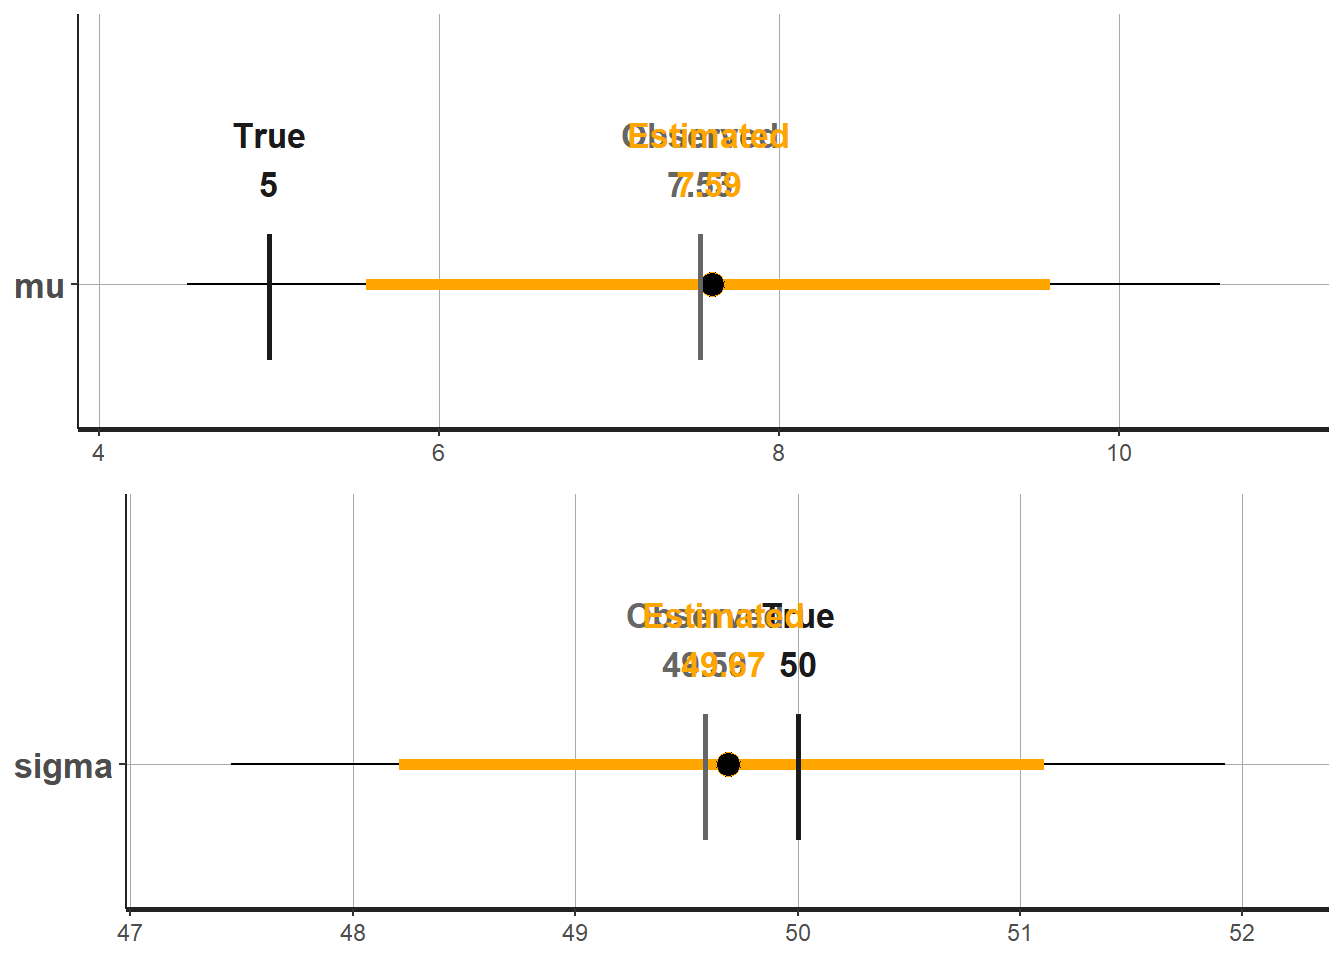
\includegraphics{_main_files/figure-latex/unnamed-chunk-21-1.pdf}

The most likely population estimate is the mean of this distribution
(e.g.~100 people, in this case).

\begin{Shaded}
\begin{Highlighting}[]
\KeywordTok{summary}\NormalTok{(x)}
\end{Highlighting}
\end{Shaded}

\begin{verbatim}
##    Min. 1st Qu.  Median    Mean 3rd Qu.    Max. 
##   63.00   93.00  100.00   99.81  106.00  141.00
\end{verbatim}

The 95\% confidence intervals for the population estimate can be
calculated as the 0.025 and 0.975 quantiles:

\begin{Shaded}
\begin{Highlighting}[]
\KeywordTok{quantile}\NormalTok{(x, }\DataTypeTok{probs=}\KeywordTok{c}\NormalTok{(}\FloatTok{0.025}\NormalTok{, }\FloatTok{0.975}\NormalTok{))}
\end{Highlighting}
\end{Shaded}

\begin{verbatim}
##  2.5% 97.5% 
##    81   120
\end{verbatim}

\subsection{Point-based: total
population}\label{point-based-total-population}

\textbf{API Endpoint:}\\
https://api.worldpop.org/v1/wopr/pointtotal

This endpoint accepts coordinates for a point location and returns the
total population. Requests to this API endpoint require the following
arguments:

\begin{itemize}
\item
  \textbf{iso3} The ISO country codes of the country to query (e.g.
  \texttt{NGA}).
\item
  \textbf{ver} The version of the population estimates to query (e.g.
  \texttt{1.2}).
\item
  \textbf{lat} The latitude of the location to query using the WGS84
  coordinate system (e.g. \texttt{11.53579}).
\item
  \textbf{lon} The longitude of the location to query using the WGS84
  coordinate system (e.g. \texttt{4.850808}).
\end{itemize}

An example of an API request:\\
https://api.worldpop.org/v1/wopr/pointtotal?iso3=NGA\&ver=1.2\&lat=11.53579\&lon=4.850808

This request returns a task identification number
\texttt{2a6a2883-3fd7-5fbf-832c-86e5f35e7c5e} that can be used to query
the result:\\
https://api.worldpop.org/v1/tasks/2a6a2883-3fd7-5fbf-832c-86e5f35e7c5e

Results for any task id from WOPR can be retrieved in this way,
regardless of the endpoint used to submit the request.

\subsection{Point-based: specific age-sex
group}\label{point-based-specific-age-sex-group}

\textbf{API Endpoint:}\\
https://api.worldpop.org/v1/wopr/pointagesex

This endpoint accepts coordinates for a point location and returns the
population size for a specified age-sex group. Requests to this API
endpoint require the following arguments:

\begin{itemize}
\item
  \textbf{iso3} The ISO country codes of the country to query (e.g.
  \texttt{NGA}).
\item
  \textbf{ver} The version of the population estimates to query (e.g.
  \texttt{1.2}).
\item
  \textbf{lat} The latitude of the location to query using the WGS84
  coordinate system (e.g. \texttt{11.53579}).
\item
  \textbf{lon} The longitude of the location to query using the WGS84
  coordinate system (e.g. \texttt{4.850808}).
\item
  \textbf{agesex} The age-sex groups for which a population estimate is
  required. This argument accepts a comma-separated vector of age-sex
  group identifiers. \texttt{f0} represents females less than one year
  old; \texttt{f1} represents females from age one to four; \texttt{f5}
  represents females from five to nine; \texttt{f10} represents females
  from 10 to 14; and so on. \texttt{m0} represents males less than one,
  etc. The full list of acceptable values:
  \texttt{m0,\ m1,\ m5,\ m10,\ m15,\ m20,\ m25,\ m30,\ m35,\ m40,\ m45,\ m50,\ m55,\ m60,\ m65,\ m70,\ m75,\ m80,\ f0,\ f1,\ f5,\ f10,\ f15,\ f20,\ f25,\ f30,\ f35,\ f40,\ f45,\ f50,\ f55,\ f60,\ f65,\ f70,\ f75,\ f80}.
\end{itemize}

An example of an API request:\\
https://api.worldpop.org/v1/wopr/pointagesex?iso3=NGA\&ver=1.2\&lat=11.53579\&lon=4.850808\&agesex=m0,m1,f0,f1

This request will return the population of children under five at the
specified point location. The task id was
\texttt{38f18d6e-d7d8-5886-828a-45c29da7f766}. This can be used to
retrieve the result:\\
https://api.worldpop.org/v1/tasks/38f18d6e-d7d8-5886-828a-45c29da7f766

\subsection{Polygon-based: total
population}\label{polygon-based-total-population}

\textbf{API Endpoint:}\\
https://api.worldpop.org/v1/wopr/polytotal

This endpoint accepts a GeoJSON representing a polygon location and
returns the total population. Requests to this API endpoint require the
following arguments:

\begin{itemize}
\item
  \textbf{iso3} The ISO country codes of the country to query (e.g.
  \texttt{NGA}).
\item
  \textbf{ver} The version of the population estimates to query (e.g.
  \texttt{1.2}).
\item
  \textbf{geojson} A GeoJSON representing the polygon location to query
  (see example below).
\end{itemize}

\begin{verbatim}
{
  "type": "FeatureCollection",
  "features": [
    {
      "type": "Feature",
      "properties": {},
      "geometry": {
        "type": "Polygon",
        "coordinates": [
          [
            [
              3.2080078125,
              7.0027636819827475
            ],
            [
              3.7902832031250004,
              7.0027636819827475
            ],
            [
              3.7902832031250004,
              7.612997502224103
            ],
            [
              3.2080078125,
              7.612997502224103
            ],
            [
              3.2080078125,
              7.0027636819827475
            ]
          ]
        ]
      }
    }
  ]
}
\end{verbatim}

An example of an API request:\\
\url{https://api.worldpop.org/v1/wopr/polytotal?iso3=NGA\&ver=1.2\&geojson}=\{``type'':``FeatureCollection'',``features'':{[}\{``type'':``Feature'',``properties'':\{\},``geometry'':\{``type'':``Polygon'',``coordinates'':{[}{[}{[}3.2080078125,7.0027636819827475{]},{[}3.7902832031250004,7.0027636819827475{]},{[}3.7902832031250004,7.612997502224103{]},{[}3.2080078125,7.612997502224103{]},{[}3.2080078125,7.0027636819827475{]}{]}{]}\}\}{]}\}

This request returns a task identification number
\texttt{06b50b9f-d94d-50b9-916a-1d34b767d00a} that can be used to query
the result:\\
https://api.worldpop.org/v1/tasks/06b50b9f-d94d-50b9-916a-1d34b767d00a

\subsection{Polygon-based: specific age-sex
group}\label{polygon-based-specific-age-sex-group}

\textbf{API Endpoint:}\\
https://api.worldpop.org/v1/wopr/polyagesex

This endpoint accepts a GeoJSON representing a polygon location and
returns the population size within a specified age-sex group. Requests
to this API endpoint require the following arguments:

\begin{itemize}
\item
  \textbf{iso3} The ISO country codes of the country to query (e.g.
  \texttt{NGA}).
\item
  \textbf{ver} The version of the population estimates to query (e.g.
  \texttt{1.2}).
\item
  \textbf{geojson} A GeoJSON representing the polygon location to query
  (see example above).
\item
  \textbf{agesex} The age-sex groups for which a population estimate is
  required. This argument accepts a comma-separated vector of age-sex
  group identifiers. The full list of acceptable values:
  \texttt{m0,\ m1,\ m5,\ m10,\ m15,\ m20,\ m25,\ m30,\ m35,\ m40,\ m45,\ m50,\ m55,\ m60,\ m65,\ m70,\ m75,\ m80,\ f0,\ f1,\ f5,\ f10,\ f15,\ f20,\ f25,\ f30,\ f35,\ f40,\ f45,\ f50,\ f55,\ f60,\ f65,\ f70,\ f75,\ f80}.
\end{itemize}

An example of an API request:\\
\url{https://api.worldpop.org/v1/wopr/polyagesex?iso3=NGA\&ver=1.2\&agesex=m0,m1,f0,f1\&geojson}=\{``type'':``FeatureCollection'',``features'':{[}\{``type'':``Feature'',``properties'':\{\},``geometry'':\{``type'':``Polygon'',``coordinates'':{[}{[}{[}3.2080078125,7.0027636819827475{]},{[}3.7902832031250004,7.0027636819827475{]},{[}3.7902832031250004,7.612997502224103{]},{[}3.2080078125,7.612997502224103{]},{[}3.2080078125,7.0027636819827475{]}{]}{]}\}\}{]}\}

This request returns a task identification number
\texttt{b6418707-d795-56ef-9d06-c469e3697782} that can be used to query
the result:\\
https://api.worldpop.org/v1/tasks/b6418707-d795-56ef-9d06-c469e3697782

Contributing

Funding for the work described in this chapter was provided by the Bill
and Melinda Gates Foundation and the United Kingdom Department for
International Development (OPP1134076, OPP1182408). Maksym Bondarenko
developed the WOPR API. This chapter was written by Doug Leasure. Andy
Tatem provides oversight of the WorldPop Research Group.

Suggested Citation

Bondarenko M, Leasure DR, Tatem AJ. 2020. Resources for Developers: WOPR
API. In \emph{WorldPop Book of Methods}. WorldPop Research Group,
University of Southampton. 26 November 2020,
\url{https://docs.worldpop.org/bookworm}

\appendix


\chapter{Census Support}\label{census-support}

\section{Introduction}\label{introduction-6}

\emph{Challenge:}\\
Census cannot always achieve national coverage because some areas may be
inaccessible to census field workers. Census results can also become
outdated, particularly in localized areas where migration is occurring.

\emph{Solution:}\\
Use statistical models to estimate populations in areas where census
results are not available or are outdated. Statistical models relate
observed population sizes from accessible areas to other data sets that
can be mapped everywhere (i.e.~in accessible and inaccessible areas).
These relationships form the basis for population estimates in
inaccessible areas.

\emph{Technical Overview:}\\
WorldPop at the University of Southampton develops customized Bayesian
statistical models for individual countries to maximize the information
gleaned from available data. These models generally estimate the number
of people in every 100 m grid cell within the area(s) of interest. Each
population estimate is accompanied by a range of uncertainty
(i.e.~confidence intervals) for a given level of confidence (e.g.~95\%
confidence). These gridded population estimates can be aggregated within
administrative units or other boundaries to derive population totals
(with confidence intervals) for larger areas. WorldPop models are
developed in the R programming language and the code can be openly
shared among stakeholders.

\section{Input Data}\label{input-data-3}

\textbf{Key data inputs:}

\begin{enumerate}
\def\labelenumi{\arabic{enumi}.}
\tightlist
\item
  Population data\\
\item
  Settlement map\\
\item
  Geospatial covariates\\
\item
  Administrative boundaries
\end{enumerate}

\subsection{Population Data}\label{population-data-1}

Population data from accessible areas are essential to be able to
estimate populations in inaccessible areas. Population data used for
modelling must include counts of people in clearly defined georeferenced
areas. A polygon shapefile with the boundary of each enumeration area
and the total population within each area would be ideal. There are a
few potential sources for these data:

\begin{itemize}
\tightlist
\item
  Partial census results\\
\item
  Microcensus surveys designed for population modelling (a random sample
  of locations where enumeration is carried out)\\
\item
  Pre-survey listing data from routine household surveys (e.g.~DHS,
  LSMS, MICS)
\end{itemize}

Point locations of buildings and/or households within enumeration areas
are sometimes collected during census and survey field work. These data
can be very useful because they provide higher resolution information
about population patterns, but they are not required. Pre-survey listing
data can be very useful, especially if surveys were recently conducted
in areas that were inaccessible to census enumerators. If pre-survey
listing data from household surveys are used, additional information
about the site selection will also be required. If the household survey
used a sampling design in which survey locations were selected with
probabilities proportional to population size (PPS), then it will be
necessary to obtain the weights used for PPS sample design.

\subsection{Settlement Map}\label{settlement-map-1}

A settlement map identifies areas where residential structures occur. It
may also classify areas into settlement types such as urban, peri-urban,
rural, slums, commercial, industrial, etc. This information may be in
the form of:

\begin{itemize}
\tightlist
\item
  Building locations (points)\\
\item
  Building footprints (polygons)\\
\item
  Gridded map identifying pixels that contain buildings (raster)
\end{itemize}

These data could be derived from several sources:

\begin{itemize}
\tightlist
\item
  Satellite imagery\\
\item
  Pre-census cartography\\
\item
  Building points and footprints can be purchased commercially
\end{itemize}

If there is no classification of settlement types available, building
points or building footprints could be directly used to identify
different settlement types based on the patterns of building locations
(building density, spacing, regularity, etc). There are also freely
available global settlement maps, but quality from global data sets
varies strongly among countries, with the smallest settlements often
missing, so this would need to be considered before committing to any
publicly available global settlement map. Additional data about each
building can be very beneficial for population modelling such as
building area, height, or use (i.e.~residential, commercial, mixed).
While these additional data would improve population estimates, they are
not required.

\subsection{Geospatial Covariates}\label{geospatial-covariates-3}

Geospatial covariates are spatial data (e.g.~GIS data) with national
coverage that describe any variable that may be correlated with
population densities.

For example, a digital map of road networks (a line shapefile) could be
used to calculate road densities which may correlate with population
densities. Or, global satellite-derived nighttime lights data sets
(raster files) may correlate with population densities in some areas.
Administrative records could also be useful such as electricity usage
for each administrative unit (polygon shapefile). Locations of public
facilities such as schools (a point shapefile) can also be very
informative. If the number of students attending each school is known,
that would also likely add to the accuracy of population estimates.

There are an almost infinite number of possible geospatial covariates.
Many of them are publicly available, so identifying these data sets is
not necessarily required to initiate population modelling. But,
identifying good quality covariates (i.e.~those that are strongly
correlated to population density) that are comprehensive with national
coverage can significantly improve the accuracy of population estimates.

Some examples include:

\begin{itemize}
\tightlist
\item
  Road networks
\item
  Intensity of nighttime lights
\item
  Electricity usage
\item
  School locations
\item
  School enrollment numbers
\item
  Health facility locations
\item
  Police station locations
\item
  Locations of large employers (factories, mines, etc.)
\item
  Average household size (aggregated, not personal data)
\item
  Average income (aggregated, not personal data)
\item
  Land cover (forest, agriculture, urban, etc.)
\item
  Terrain slope and elevation
\item
  Climate variables (temperature, precipitation)
\end{itemize}

\subsection{Administrative
Boundaries}\label{administrative-boundaries-1}

Administrative boundaries could include regions, states (provinces),
and/or local government areas. These administrative units are often
nested within one another. Administrative units can be used by the model
as a covariate to improve estimates of population densities.
Administrative units can also be used to summarize model results,
providing population totals for each administrative unit.

\section{Recommendations}\label{recommendations}

To assess the potential for hybrid census implementation for a specific
country and potential modelling methods, sharing of sample data for any
specific area relating to the above categories would be valuable. In
particular, a sample of the population data with indications of areas
that were not enumerated, and any geospatial data on settlement/building
locations would be especially useful.

\subsection*{Contributing}\label{contributing-10}
\addcontentsline{toc}{subsection}{Contributing}

This chapter was written by Doug Leasure and Andy Tatem.

\subsection*{Suggested Citation}\label{suggested-citation-10}
\addcontentsline{toc}{subsection}{Suggested Citation}

WorldPop. 2020. Hybrid Census. In: \emph{WorldPop Book of Methods}.
WorldPop Research Group, University of Southampton. 26 November 2020,
\url{https://docs.worldpop.org/bookworm}

\subsection*{References}\label{references}
\addcontentsline{toc}{subsection}{References}

\bibliography{bib/book.bib,bib/GHAv1.bib,bib/BFAv1.bib}

\end{document}
